\newpage
\section{HÀM SỐ LŨY THỪA}
\Opensolutionfile{ans}[ans/ansCD2D2-2]
\subsection{KIẾN THỨC SÁCH GIÁO KHOA CẦN NẮM}
\textbf{1. Định nghĩa:} Hàm số $y=x^{\alpha},$ với $\alpha\in\mathbb{R},$ được gọi là hàm số lũy thừa.\\
\textbf{2. Tập xác định:} Tập xác định của hàm số $y=x^{\alpha}$ là\\
$\mathbb{R}$ nếu $\alpha$ là số nguyên dương.\\
$\mathbb{R}\setminus \left\{0\right\}$với $\alpha$ nguyên âm hoặc bằng $0$;\\
$(0;+\infty)$ với $\alpha$ không nguyên.\\
\textbf{3. Đạo hàm:} Hàm số $y=x^{\alpha}, (\alpha\in\mathbb{R})$ có đạo hàm với mọi $x>0$ và $(x^{\alpha})'=\alpha\cdot x^{\alpha-1}$.\\
\textbf{4. Tính chất của hàm số lũy thừa trên khoảng $(0;+\infty)$} (khảo sát hàm lũy thừa). 
\begin{longtable}{|l|l|}
\hline
 $y=x^{\alpha},\alpha>0$  &  $y=x^{\alpha},\alpha<0$  \\
\hline
\textbf{A.} Tập khảo sát: $(0;+\infty)$.  & \textbf{A.} Tập khảo sát: $(0;+\infty)$.  \\
\hline
\textbf{B.} Sự biến thiên:& \textbf{B.} Sự biến thiên:\\ 
$y'=\alpha x^{\alpha-1}>0,\forall x>0$.&$y'=\alpha x^{\alpha-1}<0,\forall x>0$.\\
Giới hạn đặc biệt:&Giới hạn đặc biệt:\\
$\lim\limits_{x\to 0^+} x^{\alpha}=0,\lim\limits_{x\to+\infty} x^{\alpha}=+\infty$.& $\lim\limits_{x\to 0^+} x^{\alpha}=+\infty,\lim\limits_{x\to+\infty} x^{\alpha}=0$.\\
Tiệm cận: Không có  &Tiệm cận: Trục $Ox$ là tiệm cận ngang.\\
& Trục $Oy$ là tiệm cận đứng. \\
\hline
\textbf{C.} Bảng biến thiên: & \textbf{C.} Bảng biến thiên \\	
	
\begin{tikzpicture}
\tkzTabInit[espcl=3,lgt=1.5,nocadre]
{$x$/0.7,$y'$/0.7,$y$/2.1}
{$0$,$+\infty$}
\tkzTabLine{,+,}
\tkzTabVar{-/$0$,+/$+\infty$}
\end{tikzpicture}
 &
 

\begin{tikzpicture}
\tkzTabInit[espcl=3,lgt=1.5,nocadre]
{$x$/0.7,$y'$/0.7,$y$/2.1}
{$0$,$+\infty$}
\tkzTabLine{,-,}
\tkzTabVar{+/$+\infty$,-/$0$}
\end{tikzpicture}
\\
\hline
\end{longtable}
\textbf{D. Đồ thị}
\begin{center}
	\begin{tikzpicture}[>=stealth,scale=1.2, line join=round, line cap=round]
	\def\a{-1} \def\b{3} \def\c{-1} % Hệ số
	\def\xmin{-3} \def\xmax{4}
	\def\ymin{-1.6}\def\ymax{3.5} 
	\draw[->] (-1,0)--(\xmax,0) node [below]{$x$};
	\draw (0,1)--(\xmax,1) node [above]{\footnotesize $\alpha =0$};
	\draw[->] (0,-0.5)--(0,\ymax) node [left]{$y$};
	\draw[dashed](1,0)--(1,1);
	\node at (0,0) [above left]{\footnotesize $O$};
	\node at (0,1) [left]{\footnotesize $1$};
	\node at (1,0) [below]{\footnotesize $1$};
	\node at (4,0.1) [above]{\footnotesize $\alpha <0$};
	\node at (4,2.2) [above]{\footnotesize $0<\alpha <1$};
	\node at (4,3.2) [above]{\footnotesize $\alpha =1$};
	\node at (2.3,3.5) [above]{\footnotesize $\alpha >1$};
	\clip (\xmin+0.1,\ymin+0.1) rectangle (\xmax,\ymax-0.1);
	\draw[samples=200,domain=0.01:5.5,smooth,variable=\x] plot (\x,{(\x)^1.6});
	\draw[samples=200,domain=0.01:5.5,smooth,variable=\x] plot (\x,{(\x)^0.6});
	\draw[samples=200,domain=0.01:5.5,smooth,variable=\x] plot (\x,{(\x)^1});
	\draw[samples=200,domain=0.01:5.8,smooth,variable=\x] plot (\x,{(1/((\x)^1.2)}) node[above]{$\alpha<0$};
	\end{tikzpicture}
\end{center}
Đồ thị của hàm số lũy thừa $y=x^{\alpha}$ luôn đi qua điểm $I(1;1)$.\\
\textbf{Lưu ý:} Khi khảo sát hàm số lũy thừa với số mũ cụ thể, ta phải xét hàm số đó trên toàn bộ tập xác định của nó. Chẳng hạn: $y=x^3, y=x^{-2}, y=x^{\pi}$.
\subsection{Phân loại và phương pháp giải bài tập}
\begin{dang}{Tập xác định của hàm số lũy thừa, hàm số vô tỷ}
	Phương pháp giải.\\
	- Tự luận thuần túy:\\
	Xét hàm số $y=[f(x)]^{\alpha}$.\\
	Khi $\alpha$ nguyên dương: hàm số xác định khi và chỉ khi $f(x)$ xác định.\\
	Khi $\alpha$ nguyên âm: hàm số xác định khi và chỉ khi $f(x)\neq 0$.\\
	Khi $\alpha$ không nguyên: hàm số xác định khi và chỉ khi $f(x)>0$.\\
	- Sử dụng MTBT:\\
	MODE 7 $\to$ NHẬP HÀM $\to$ START: a $\to$ END: b $\to$ STEP: (b-a): 19.
\end{dang}

\subsubsection{Các ví dụ}
\begin{vd}%[2D2B2-1]%[Đào Trung Kiên]%Ví dụ 1: 
	Tìm tập xác định $D$ của hàm số $y=\left(6x^2-x-5\right)^3$.
	\loigiai{
		Hàm số xác định khi và chỉ khi $6x^2-x-5$ xác định $\Leftrightarrow x\in\mathbb{R}$.}
\end{vd}
\begin{vd}%[2D2B2-1]%[Đào Trung Kiên]%Ví dụ 2: 
	Tìm tập xác định $D$ của hàm số $y=\left(x^2-1\right)^{-8}$.
	\loigiai{
		Hàm số xác định khi và chỉ khi $x^2-1\neq 0\Leftrightarrow x\neq\pm 1$.}
\end{vd}
\begin{vd}%[2D2B2-1]%[Đào Trung Kiên]%Ví dụ 3: 
	Tìm tập xác định $D$ của hàm số $y=(x+1)^{\tfrac{3}{4}}$.
	\loigiai{
		Hàm số xác định khi và chỉ khi $x+1>0\Leftrightarrow x >-1$.}
\end{vd}
\begin{vd}%[2D2B2-1]%[Đào Trung Kiên]%Ví dụ 4: 
	Tìm tập xác định $D$ của hàm số $y=\left(\sqrt{x-1}+2018\right)^{-\tfrac{5}{2}}$.
	\loigiai{
		Hàm số xác định khi và chỉ khi $x-1\geq 0\Leftrightarrow x\geq 1$.}
\end{vd}
\begin{vd}%[2D2B2-1]%[Đào Trung Kiên]%Ví dụ 5: 
	Tìm tập xác định $D$ của hàm số $y=\left(\dfrac{2x-3}{x^2-3x+2}\right)^3$.
	\loigiai{
		Hàm số xác định khi và chỉ khi $\dfrac{2x-3}{x^2-3x+2}$ xác định $\Leftrightarrow x^2-3x+2\neq 0\Leftrightarrow\heva{&x\neq 1\\&x\neq 2.}$ }
\end{vd}
\begin{vd}%[2D2B2-1]%[Đào Trung Kiên]%Ví dụ 6: 
	Tìm tập xác định của hàm số $y=\left(\dfrac{x-4}{x+1}\right)^{e-1}$.
	\loigiai{
		Hàm số xác định khi và chỉ khi $\dfrac{x-4}{x+1}>0\Leftrightarrow x\in (-\infty;-1)\cup (4;+\infty)$.}
\end{vd}
\subsubsection{Câu hỏi trắc nghiệm}
\begin{ex}%[2D2B2-1]%[Đào Trung Kiên]%Câu 1.
	Tìm tập xác định $D$ của hàm số $y=x^m$, với $m$ là một số nguyên dương. 
	\choice
	{\True $\mathscr{D}=\mathbb{R}$}
	{$\mathscr{D}=\mathbb{R}\setminus\{0\}$}
	{$\mathscr{D}=(-\infty; 0)$}
	{$\mathscr{D}=(0;+\infty)$}
	\loigiai{
		Hàm số xác định $\forall x\in\mathbb{R}$.}
\end{ex}
\begin{ex}%[2D2B2-1]%[Đào Trung Kiên]%Câu 2.
	Tìm tập xác định $D$ của hàm số $y=x^{\alpha}$, với $\alpha$ không nguyên. 
	\choice
	{$\mathscr{D}=\mathbb{R}$}
	{$\mathscr{D}=\mathbb{R}\setminus\{0\}$}
	{$\mathscr{D}=(-\infty; 0)$}
	{\True $\mathscr{D}=(0;+\infty)$}
	\loigiai{
		Hàm số xác định $\forall x\in(0;+\infty)$.}
\end{ex}
\begin{ex}%[2D2B2-1]%[Đào Trung Kiên]%Câu 3.
	Tìm điều kiện của $x$ để hàm số $y=x^{\pi+1}$ có nghĩa. 
	\choice
	{$x\in\mathbb{R}$}
	{$x\neq 0$}
	{$x<0$}
	{\True $x>0$}
	\loigiai{
		Hàm số xác định $\forall x\in(0;+\infty)$.}
\end{ex}
\begin{ex}%[2D2B2-1]%[Đào Trung Kiên]%Câu 4.
	Tìm điều kiện của $x$ để hàm số $y=x^{\tfrac{2}{5}}$ có nghĩa. 
	\choice
	{$x\in\mathbb{R}$}
	{$x\neq 0$}
	{$x<0$}
	{\True $x>0$}
	\loigiai{
		Hàm số xác định $\forall x\in(0;+\infty)$.}
\end{ex}
\begin{ex}%[2D2B2-1]%[Đào Trung Kiên]%Câu 5.
	Tìm tập xác định $D$ của hàm số $y=\sqrt[5]{x}$. 
	\choice
	{\True $\mathscr{D}=\mathbb{R}$}
	{$\mathscr{D}=\mathbb{R}\setminus\{0\}$}
	{$\mathscr{D}=[0;+\infty)$}
	{$\mathscr{D}=(0;+\infty)$}
	\loigiai{
		Hàm số xác định $\forall x\in\mathbb{R}$.}
\end{ex}
\begin{ex}%[2D2B2-1]%[Đào Trung Kiên]%Câu 6.
	Tìm tập xác định $D$ của hàm số $y=(1+x-x^2)^m$, với $m$ là một số nguyên dương. 
	\choice
	{\True $\mathscr{D}=\mathbb{R}$}
	{$\mathscr{D}=\mathbb{R}\setminus\{0\}$}
	{$\mathscr{D}=(-\infty; 0)$}
	{$\mathscr{D}=(0;+\infty)$}
	\loigiai{
		Hàm số xác định $\forall x\in\mathbb{R}$.}
\end{ex}
\begin{ex}%[2D2B2-1]%[Đào Trung Kiên]%Câu 7.
	Tìm tập xác định $D$ của hàm số $y=(2x-4)^{-2018}$. 
	\choice
	{$\mathscr{D}=\mathbb{R}$}
	{\True $\mathscr{D}=\mathbb{R}\setminus\{0\}$}
	{$\mathscr{D}=\mathbb{R}\setminus\{2\}$}
	{$\mathscr{D}=(2;+\infty)$}
	\loigiai{
		Hàm số xác định $\forall x\in\mathbb{R}\setminus\{0\}$.}
\end{ex}
\begin{ex}%[2D2B2-1]%[Đào Trung Kiên]%Câu 8.
	Tìm tập xác định $D$ của hàm số $y=(1-2x)^{\sqrt{3}-1}$. 
	\choice
	{$\mathscr{D}=\left(\dfrac{1}{2};+\infty\right)$}
	{$\mathscr{D}=\mathbb{R}\setminus\left\{\dfrac{1}{2}\right\}$}
	{\True $\mathscr{D}=\left(-\infty;\dfrac{1}{2}\right)$}
	{$\mathscr{D}=(0;+\infty)$}
	\loigiai{
		Hàm số xác định khi và chỉ khi $1-2x>0\Leftrightarrow x\in (-\infty;\dfrac{1}{2})$.}
\end{ex}
\begin{ex}%[2D2B2-1]%[Đào Trung Kiên]%Câu 9.
	Tìm tập xác định $D$ của hàm số $y=(5x+10)^{\alpha}$, với $\alpha\in\mathbb{Q}$. 
	\choice
	{$\mathscr{D}=\mathbb{R}$}
	{\True $\mathscr{D}=(-2;+\infty)$}
	{$\mathscr{D}=(-\infty;-2)$}
	{$\mathscr{D}=\mathbb{R}\setminus\{-2\}$}
	\loigiai{
		Hàm số xác định khi và chỉ khi $5x+10>0\Leftrightarrow x\in (-2;+\infty)$.}
\end{ex}
\begin{ex}%[2D2B2-1]%[Đào Trung Kiên]%Câu 10.
	Tìm tập xác định $D$ của hàm số $y=\sqrt{4-3x}$. 
	\choice
	{$\mathscr{D}=\left(-\infty;\dfrac{4}{3}\right)$}
	{\True $\mathscr{D}=\left(-\infty;\dfrac{4}{3}\right]$}
	{$\mathscr{D}=\left[\dfrac{4}{3};+\infty\right)$}
	{$\mathscr{D}=\mathbb{R}\setminus\left\{\dfrac{4}{3}\right\}$}
	\loigiai{
		Hàm số xác định khi và chỉ khi $4-3x\geq 0\Leftrightarrow x\in\left(-\infty;\dfrac{4}{3}\right]$.}
\end{ex}
\begin{ex}%[2D2B2-1]%[Đào Trung Kiên]%Câu 11.
	Tìm tập xác định $D$ của hàm số $y=\left(1-x^2\right)^{-2018}+2x-4$. 
	\choice
	{\True $\mathscr{D}=\mathbb{R}\setminus\{-1; 1\}$}
	{$\mathscr{D}=(-1; 1)$}
	{$\mathscr{D}=[-1; 1]$}
	{$\mathscr{D}=\mathbb{R}\setminus\{2\}$}
	\loigiai{
		Hàm số xác định khi và chỉ khi $1-x^2\neq 0\Leftrightarrow x\neq\pm 1$.\\
		Vậy tập xác định của hàm số là $\mathscr{D}=\mathbb{R}\setminus\{-1; 1\}$.}
\end{ex}
\begin{ex}%[2D2B2-1]%[Đào Trung Kiên]%Câu 12.
	Tìm tập xác định $D$ của hàm số $y=\left(1+x-2x^2\right)^{\sqrt{2}+2}+2x^2+x-3$. 
	\choice
	{$\mathscr{D}=\mathbb{R}\setminus\left\{-\dfrac{1}{2}; 1\right\}$}
	{\True $\mathscr{D}=\left(-\dfrac{1}{2}; 1\right)$}
	{$\mathscr{D}=\left[-\dfrac{1}{2}; 1\right]$}
	{$\mathscr{D}=\mathbb{R}$}
	\loigiai{
		Hàm số xác định khi và chỉ khi $1+x-2x^2>0\Leftrightarrow-\dfrac{1}{2}<x<1$.\\
		Vậy tập xác định của hàm số là $\mathscr{D}=\left(-\dfrac{1}{2}; 1\right)$.}
\end{ex}
\begin{ex}%[2D2B2-1]%[Đào Trung Kiên]%Câu 13.
	Tìm tập xác định $D$ của hàm số $y=\left(x^2-2x+1\right)^{e+1}+x^2-3x-4$. 
	\choice
	{\True $\mathscr{D}=\mathbb{R}\setminus\{1\}$}
	{$\mathscr{D}=(-\infty; 1)$}
	{$\mathscr{D}=(1;+\infty)$}
	{$\mathscr{D}=\mathbb{R}$}
	\loigiai{
		Hàm số xác định khi và chỉ khi $x^2-2x+1>0\Leftrightarrow x\neq 1$.\\
		Vậy tập xác định của hàm số là $\mathscr{D}=\mathbb{R}\setminus\{1\}$.}
\end{ex}
\begin{ex}%[2D2B2-1]%[Đào Trung Kiên]%Câu 14.
	Tìm tập xác định $D$ của hàm số $y=\sqrt{\dfrac{x-1}{x+1}}+x-2$. 
	\choice
	{$\mathscr{D}=(-1; 1)$}
	{\True $\mathscr{D}=(-\infty;-1)\cup[1;+\infty)$}
	{$\mathscr{D}=(-\infty;-1)\cup(1;+\infty)$}
	{$\mathscr{D}=(-\infty;-1]\cup[1;+\infty)$}
	\loigiai{
		Hàm số xác định khi và chỉ khi $\dfrac{x-1}{x+1}\geq 0\Leftrightarrow\hoac{&x <-1\\&x\geq 1.}$ \\
		Vậy tập xác định của hàm số là $\mathscr{D}=(-\infty;-1)\cup[1;+\infty)$.}
\end{ex}
\begin{ex}%[2D2B2-1]%[Đào Trung Kiên]%Câu 15.
	Tìm tập xác định $D$ của hàm số $y=\sqrt{4-x^2}+\sqrt[3]{\dfrac{x+1}{x-1}}+x+1$. 
	\choice
	{$\mathscr{D}=[-2; 2]$}
	{\True $\mathscr{D}=[-2; 2]\setminus\{1\}$}
	{$\mathscr{D}=(-\infty;-2)\cup(2;+\infty)$}
	{$\mathscr{D}=(-2; 2)\setminus\{1\}$}
	\loigiai{
		Hàm số xác định khi và chỉ khi $\heva{&4-x^2\geq 0\\&x\neq 1}\Leftrightarrow\heva{&-2\leq x\leq 2\\&x\neq 1.}$ \\
		Vậy tập xác định của hàm số là $\mathscr{D}=[-2; 2]\setminus\{1\}$.}
\end{ex}
\begin{ex}%[2D2B2-1]%[Đào Trung Kiên]%Câu 16.
	Tìm tập xác định $D$ của hàm số $y=(x-2)^{\sqrt{5}}+\left(x^2-9\right)^{\tfrac{3}{5}}+x^2-5x-2$. 
	\choice
	{$\mathscr{D}=(-\infty;-3)\cup(3;+\infty)$}
	{$\mathscr{D}=(2;+\infty)$}
	{\True $\mathscr{D}=(3;+\infty)$}
	{$\mathscr{D}=\mathbb{R}\setminus\{-3, 3, 2\}$}
	\loigiai{
		Hàm số xác định khi và chỉ khi $\heva{&x-2>0\\&x^2-9>0}\Leftrightarrow\heva{&x>2\\&\hoac{&x <-3\\&x>3}}\Leftrightarrow x>3$.\\
		Vậy tập xác định của hàm số là $\mathscr{D}=(3;+\infty)$.}
\end{ex}
\begin{ex}%[2D2B2-1]%[Đào Trung Kiên]%Câu 17.
	Tìm tập xác định $D$ của hàm số $y=\sqrt{\dfrac{x^2-3x+2}{3-x}}+(2x-5)^{\sqrt{7}+1}-3x-11$. 
	\choice
	{\True $\mathscr{D}=\left(\dfrac{5}{2}; 3\right)$}
	{$\mathscr{D}=\left(\dfrac{5}{2}; 3\right]$}
	{$\mathscr{D}=\left(\dfrac{5}{2};+\infty\right)$}
	{$\mathscr{D}=(2; 3)$}
	\loigiai{
		Hàm số xác định khi và chỉ khi $\heva{&\dfrac{x^2-3x+2}{3-x}\geq 0\\&2x-5>0}\Leftrightarrow\heva{&\hoac{&x\leq 1\\&2\leq x<3}\\&x>\dfrac{5}{2}}\Leftrightarrow\dfrac{5}{2}<x<3$.\\
		Vậy tập xác định của hàm số là $\mathscr{D}=\left(\dfrac{5}{2}; 3\right)$.}
\end{ex}
\begin{ex}%[2D2B2-1]%[Đào Trung Kiên]%Câu 18.
	Tìm tập xác định $D$ của hàm số $y=\sqrt{25-x^2}+\sqrt[3]{x^2+3x-4}-\left(x^2-1\right)^{\pi-e}+2x-7$. 
	\choice
	{$\mathscr{D}=(-5;-1)\cup(1; 5)$}
	{\True $\mathscr{D}=[-5;-1)\cup(1; 5]$}
	{$\mathscr{D}=[-5; 5]$}
	{$\mathscr{D}=(-\infty;-1)\cup(1;+\infty)$}
	\loigiai{
		Hàm số xác định khi và chỉ khi $\heva{&25-x^2\geq 0\\&x^2-1>0}\Leftrightarrow\heva{&-5\leq x\leq 5\\&\hoac{&x <-1\\&x>1}}\Leftrightarrow\hoac{&-5\leq x <-1\\&1<x\leq 5.}$ \\
		Vậy tập xác định của hàm số là $\mathscr{D}=[-5;-1)\cup(1; 5]$.}
\end{ex}
\begin{ex}%[2D2B2-1]%[Đào Trung Kiên]%Câu 19.
	Tìm tập xác định $D$ của hàm số $y=\left(x^2-5x+4\right)^{\sqrt{2}-3}-\sqrt{x^2+3x+7}+x^{-3}+x^2-2x+1$. 
	\choice
	{\True $\mathscr{D}=(-\infty; 1)\cup(4;+\infty)\setminus\{0\}$}
	{$\mathscr{D}=(-\infty; 1)\cup(4;+\infty)$}
	{$\mathscr{D}=(1; 4)$}
	{$\mathscr{D}=[1; 4]$}
	\loigiai{
		Hàm số xác định khi và chỉ khi $\heva{&x^2-5x+4>0\\&x\neq 0}\Leftrightarrow\heva{&\hoac{&x<1\\&x>4}\\&x\neq 0.}$ \\
		Vậy tập xác định của hàm số là $\mathscr{D}=(-\infty; 1)\cup(4;+\infty)\setminus\{0\}$.}
\end{ex}
\begin{vd}%[2D2B2-1]%[Đào Trung Kiên]%Câu 20.
	Tìm tập xác định $D$ của hàm số $y=\left(\dfrac{x+2}{x-2}\right)^{-2018}-3\left(16-x^2\right)^{1-\sqrt{8}}+3$. 
	\choice
	{$\mathscr{D}=(-4; 4)\setminus\{2\}$}
	{\True $\mathscr{D}=(-4; 4)\setminus\{-2, 2\}$}
	{$\mathscr{D}=[-4; 4]$}
	{$\mathscr{D}=(-4; 4)\setminus\{-2\}$}
	\loigiai{
		Hàm số xác định khi và chỉ khi $\heva{&x+2\neq 0\\&x-2\neq 0\\&16-x^2>0}\Leftrightarrow\heva{&x\neq-2\\&x\neq 2\\&-4<x<4.}$ \\
		Vậy tập xác định của hàm số là $\mathscr{D}=(-4; 4)\setminus\{-2, 2\}$.}
\end{vd}
\begin{dang}{Đạo hàm, Max – Min của hàm số lũy thừa}
\end{dang}
\textbf{2. 1. Đạo hàm của hàm số luỹ thừa.}\\
\textbf{Loại 1:} Tính đạo hàm của hàm số lũy thừa.\\
a) Phương pháp giải.\\
- Tự luận thuần túy: Dựa vào công thức đạo hàm.\\
$\left(x^{\alpha}\right)'=\alpha\cdot x^{\alpha-1}$.\\
$\left(u^{\alpha}\right)'=\alpha\cdot u^{\alpha-1}\cdot u'$.\\
Và các công thức tính đạo hàm đã học.\\
- Trắc nghiệm: Dùng Casio.\\
$Shift\dfrac{d}{\mathrm{\,d}x} (f(x))\bigg|_{x=x_0}-f'(x_0)\approx 0$ (thường ra số có dạng $a.10^{-n}$ với $n$ nguyên dương).\\
Hoặc $\dfrac{Shift\dfrac{d}{\mathrm{\,d}x}{(f(x))}\bigg|_{x=x_0}}{f'(x_0)}\approx 1$.\\
\textbf{Loại 2:} Tính đạo hàm của hàm số tại một điểm.\\
a) Phương pháp giải.\\
- Tự luận thuần túy:\\
+ Tính đạo hàm của hàm số tại $x\in \mathscr{D}$.\\
+ Thay $x=x_0$ vào $f'(x)$.\\
- Trắc nghiệm: Dùng Casio $Shift\dfrac{d}{\mathrm{\,d}x} (f(x))\bigg|_{x=x_0}$.\\
Loại 3: Tính đạo hàm cấp cao của hàm số lũy thừa.\\
a) Phương pháp giải.\\
- Tự luận thuần túy:\\
+ Dựa vào định nghĩa đạo hàm cấp cao $f^{(n)}(x)=\left(f^{(n-1)}(x)\right)'$.\\
\textbf{2. 2. Max - min của hàm số luỹ thừa.}\\
\textbf{a) Phương pháp giải.}\\
- Tự luận thuần túy:\\
Nếu hàm số đơn điệu trên một đoạn thì GTLN, GTNN đạt được tại các đầu mút của đoạn.\\
Nếu hàm số không đơn điệu thì tiến hành việc tìm GTLN, GTNN theo quy tắc.\\
1. Tìm các điểm x1, x2, …, xn trên các khoảng (a;b), tại đó f'(x) bằng 0 hoặc f'.\\
2. Tính f(a), f(x1), f(x2),…, f(xn), f(b).\\
3. Tìm số lớn nhất $M$ và số nhỏ nhất $m$ trong các số trên. Ta có\\
	$M=\max\limits_{[a;b]} f(x),m=\min\limits_{[a;b]} f(x)$.\\
- Sử dụng MTCT:\\
MODE 7 $\to$ NHẬP HÀM $\to$ START: a $\to$ END: b $\to$ STEP: (b-a): 19.
\subsubsection{Các ví dụ}
\begin{vd}%[2D2B2-2]%[Đào Trung Kiên]%Ví dụ 1: 
	Tính đạo hàm của hàm số $y=x^9$.
	\loigiai{
		Áp dụng công thức ta có $(x^9)'=9\cdot x^8$.}
\end{vd}
\begin{vd}%[2D2B2-2]%[Đào Trung Kiên]%Ví dụ 2: 
	Tính đạo hàm của hàm số $y=x^{-4}$.
	\loigiai{
		Áp dụng công thức $\left(x^{-4}\right)'=-4\cdot x^{-5}$.}
\end{vd}
\begin{vd}%[2D2B2-2]%[Đào Trung Kiên]%Ví dụ 3: 
	Tính đạo hàm của hàm số $y=(3-x^2)^{-\tfrac{4}{3}}$.
	\loigiai{
		Áp dụng công thức $\left(u^{\alpha}\right)'=\alpha\cdot u^{\alpha-1}\cdot u'$.\\
		$y'=\dfrac{-4}{3}(3-x^2)^{\tfrac{-7}{3}}\cdot (3-x^2)'=\dfrac{-4}{3}(3-x^2)^{\tfrac{-7}{3}}(-2x)=\dfrac{8}{3}x(3-x^2)^{\tfrac{-7}{3}}$.}
\end{vd}
\begin{vd}%[2D2B2-2]%[Đào Trung Kiên]%Ví dụ 4: 
	Tính đạo hàm của hàm số $y=(x-1)^{\tfrac{1}{3}}$ tại điểm $x=2$.
	\loigiai{
		Áp dụng công thức $\left(u^{\alpha}\right)'=\alpha\cdot u^{\alpha-1}\cdot u'$.\\
		$y'=\dfrac{1}{3}(x-1)^{\tfrac{-2}{3}}\cdot (x-1)'=\dfrac{1}{3}(x-1)^{\tfrac{-2}{3}}\times 1=\dfrac{1}{3}(x-1)^{\tfrac{-2}{3}}$.\\
		$y''(2)=\dfrac{1}{3}(2-1)^{\tfrac{-2}{3}}=\dfrac{1}{3}$.}
\end{vd}
\begin{vd}%[2D2B2-2]%[Đào Trung Kiên]%Ví dụ 5: 
	Cho hàm số $y=x^{\tfrac{\pi}{2}}$ có đồ thị $(C)$. Lấy $M\in(C)$ có hoành độ $x_0=1$. Tính hệ số góc của tiếp tuyến của $(C)$ tại $M$.
	\loigiai{
		Hệ số góc của tiếp tuyến của $(C)$ tại $M$ là $y'(1)$.\\
		Áp dụng công thức $\left(x^{\alpha}\right)'=\alpha\cdot x^{\alpha-1}$.\\
		$y'=\dfrac{\pi}{2}x^{\tfrac{\pi}{2}-1}\Rightarrow y'(1)=\dfrac{\pi}{2}\cdot 1^{\tfrac{\pi}{2}-1}=\dfrac{\pi}{2}$.}
\end{vd}
\begin{vd}%[2D2B2-2]%[Đào Trung Kiên]%Ví dụ 6: 
	Tính đạo hàm của hàm số $y=(5-x)^{\sqrt{3}}$ tại điểm $x=4$.
	\loigiai{
		Áp dụng công thức $\left(u^{\alpha}\right)'=\alpha\cdot u^{\alpha-1}\cdot u'$.\\
		$y'=\sqrt{3}(5-x)^{\sqrt{3}-1}(5-x)'=-\sqrt{3}\cdot (5-x)^{\sqrt{3}-1}$. $\Rightarrow y'(4)=-\sqrt{3}\cdot (5-4)^{\sqrt{3}-1}=-\sqrt{3}$.}
\end{vd}
\begin{vd}%[2D2B2-2]%[Đào Trung Kiên]%Ví dụ 7: 
	Cho hàm số $y=(4-x^2)^3$. Tính $y''(1)$.
	\loigiai{
		Áp dụng công thức $\left(u^{\alpha}\right)'=\alpha\cdot u^{\alpha-1}\cdot u'$.\\
		$y'=3\cdot (4-x^2)^2(4-x^2)'=-6x(4-x^2)^2$.\\
		Dùng công thức $(u\cdot v)'=u'v+uv'$.\\
		$y''=-6(4-x^2)^2-6x\cdot 2(4-x^2)(-2x)=6(4-x^2)(10x^2-24)$ \\
		$\Rightarrow y''(1)=6(4-1^2)(10\cdot 1^2-24)=-252$.}
\end{vd}
\begin{vd}%[2D2B2-2]%[Đào Trung Kiên]%Ví dụ 8: 
	Tìm giá trị lớn nhất $M$ của hàm số $y=(x+1)^{\tfrac{3}{2}}$ trên đoạn $[3;15]$.
	\loigiai{
		$y'=\dfrac{3}{2}(x+1)^{\tfrac{1}{2}}>0,\forall x\in[3;15]$. Hàm số đạt giá trị lớn nhất tại $x=15\Rightarrow M=y(15)=64$.}
\end{vd}
\begin{vd}%[2D2B2-2]%[Đào Trung Kiên]%Ví dụ 9: 
	Tìm $m$ để hàm số $y=(x+m)^3$ đạt giá trị lớn nhất bằng 8 trên đoạn $[1;2]$.
	\loigiai{
		$y'=3(x+m)^2\geq 0,\forall x\in[1;2]\Rightarrow$ Hàm số đạt GTLN tại $x=2$ \\
		$ \Rightarrow y(2)=8\Leftrightarrow(2+m)^3=8\Leftrightarrow m=0 $.}
\end{vd}
\subsubsection{Câu hỏi trắc nghiệm}
\begin{ex}%[2D2B2-2]%[Đào Trung Kiên]%Câu 1.
	Đạo hàm của hàm số $y=(3-x^2)^{-\tfrac{4}{3}}$ là
	\choice
	{\True $\dfrac{8}{3}x\left(3-x^2\right)^{-\tfrac{7}{3}}$}
	{$-\dfrac{4}{3}x^2\left(3-x^2\right)^{-\tfrac{7}{3}}$}
	{$-\dfrac{8}{3}x\left(3-x^2\right)^{-\tfrac{7}{3}}$}
	{$-\dfrac{4}{3}\left(3-x^2\right)^{-\tfrac{7}{3}}$}
	\loigiai{
		$y=(x-1)^{\tfrac{1}{3}}\Rightarrow y'=\dfrac{1}{3}(x-1)'\cdot (x-1)^{\tfrac{1}{3}-1}=\dfrac{1}{3}(x-1)^{-\tfrac{2}{3}}=\dfrac{1}{3\sqrt[3]{(x-1)^2}}$.}
\end{ex}
\begin{ex}%[2D2B2-2]%[Đào Trung Kiên]%Câu 2.
	Hàm số $y=\left(3-x^2\right)^{-\tfrac{4}{3}}$ có đạo hàm trên khoảng $\left(-\sqrt{3};\sqrt{3}\right)$ là
	\choice
	{$y'=-\dfrac{4}{3}\left(3-x^2\right)^{-\tfrac{7}{3}}$}
	{\True $y'=\dfrac{8}{3}x\left(3-x^2\right)^{-\tfrac{7}{3}}$}
	{$y'=-\dfrac{8}{3}x\left(3-x^2\right)^{-\tfrac{7}{3}}$}
	{$y'=-\dfrac{4}{3}x^2\left(3-x^2\right)^{-\tfrac{7}{3}}$}
	\loigiai{
		Cách 1: Ta có $y=\left(3-x^2\right)^{=\dfrac{4}{3}}\Rightarrow y'=\dfrac{8}{3}x\left(3-x^2\right)^{-\tfrac{7}{3}}$.\\
		Cách 2.
		Cách 2: Dùng máy tính Casio tính đạo hàm của hàm số $y=\left(3-x^2\right)^{-\tfrac{4}{3}}$ tại $x_0=1.3$\\
		Thay $x_0=1.3$ vào từng phương án rồi so sánh với kết quả trên để chọn ra phương án đúng(nếu có nhiều hơn $1$ phương án đúng thì chọn giá trị $x_0$ khác)}
\end{ex}
\begin{ex}%[2D2B2-2]%[Đào Trung Kiên]%Câu 3.
	Đạo hàm của hàm số $y=\left(x^2+3\right)^{\tfrac{1}{3}}$ là
	\choice
	{$y'=\dfrac{1}{3}\left(x^2+3\right)^{-\tfrac{2}{3}}$}
	{\True $y'=\dfrac{2x}{3}\left(x^2+3\right)^{-\tfrac{2}{3}}$}
	{$y'=2x\left(x^2+3\right)^{\tfrac{1}{3}}\ln\left(x^2+3\right)$}
	{$y'=\left(x^2+3\right)^{\tfrac{1}{3}}\ln\left(x^3+3\right)$}
	\loigiai{
		$y'=\dfrac{1}{3}\left(x^2+3\right)^{-\tfrac{2}{3}}\left(x^2+3\right)'=\dfrac{2}{3}x\left(x^2+3\right)^{-\tfrac{2}{3}}$.\\
		Cách 2: Dùng máy tính Casio tính đạo hàm của hàm số $y=\left(x^2+3\right)^{\tfrac{1}{3}}$ tại $x_0=2$\\
		Thay $x_0=2$ vào từng phương án rồi so sánh với kết quả trên để chọn ra phương án đúng(nếu có nhiều hơn $1$ phương án đúng thì chọn giá trị $x_0$ khác).}
\end{ex}
\begin{ex}%[2D2B2-2]%[Đào Trung Kiên]%Câu 4.
	Đạo hàm của hàm số $y=\left(x^2+x\right)^{\alpha}$ là
	\choice
	{$2\alpha\left(x^2+1\right)^{\alpha-1}$}
	{\True $\alpha\left(x^2+x\right)^{\alpha-1}(2x+1)$}
	{$\alpha\left(x^2+x\right)^{\alpha+1}(2x+1)$}
	{$\alpha\left(x^2+x\right)^{\alpha-1}$}
	\loigiai{
		Theo công thức ta có\\
		$y'=\left(\left(x^2+x\right)^{\alpha}\right)'=\alpha\left(x^2+x\right)'\left(x^2+x\right)^{\alpha-1}=\alpha(2x+1)\left(x^2+x\right)^{\alpha-1}$.}
\end{ex}
\begin{ex}%[2D2B2-2]%[Đào Trung Kiên]%Câu 5.
	Đạo hàm của hàm số $y=\sqrt{4x^2-3x-1}$ là
	\choice
	{$\dfrac{1}{2\sqrt{4x^2-3x-1}}$}
	{$\dfrac{8x-3}{\sqrt{4x^2-3x-1}}$}
	{\True $\dfrac{8x-3}{2\sqrt{4x^2-3x-1}}$}
	{$\dfrac{4x-3}{2\sqrt{4x^2-3x-1}}$}
	\loigiai{
		Theo công thức $\left(\sqrt{u(x)}\right)'=\dfrac{u'(x)}{2\sqrt{u(x)}}$ nên.\\
		$y'=\left(\sqrt{4x^2-3x-1}\right)'=\dfrac{\left(4x^2-3x-1\right)'}{2\sqrt{4x^2-3x-1}}=\dfrac{8x-3}{2\sqrt{4x^2-3x-1}}$.\\
		Cách 2: Dùng máy tính Casio tính đạo hàm của hàm số $y=\sqrt{4x^2-3x-1}$ tại $x_0=2$.\\
	Thay $x_0=2$ vào từng phương án rồi so sánh với kết quả trên để chọn ra phương án đúng(nếu có nhiều hơn $1$ phương án đúng thì chọn giá trị $x_0$ khác).}
\end{ex}
\begin{ex}%[2D2B2-2]%[Đào Trung Kiên]%Câu 6.
	(THPT Mỹ Đức A, Hà Nội) Tính đạo hàm của hàm số $y=\left(2x^2-3x+2\right)^{\tfrac{1}{3}}$. 
	\choice
	{\True $y'=\dfrac{4x-3}{3\sqrt[3]{\left(2x^3-3x+2\right)^2}}$}
	{$y'=\dfrac{4x-3}{3\sqrt[]{\left(2x^3-3x+2\right)^2}}$}
	{$y'=\dfrac{4x-3}{3\sqrt[3]{2x^2-3x+2}}$}
	{$y'=\dfrac{4x-3}{\sqrt[3]{\left(2x^3-3x+2\right)^2}}$}
	\loigiai{
		Cách 1: $y'=\dfrac{1}{3}\left(2x^2-3x+2\right)'\left(2x^2-3x+2\right)^{-\dfrac{2}{3}}=\dfrac{4x-3}{3\sqrt[3]{\left(2x^2-3x+2\right)^2}}$.\\
	$y=\sqrt{4x^2-3x-1}$.\\
	Cách 2: Dùng máy tính Casio tính đạo hàm của hàm số $y=\left(2x^2-3x+2\right)^{\tfrac{1}{3}}$ tại $x_0=2$.\\
Thay $x_0=2$ vào từng phương án rồi so sánh với kết quả trên để chọn ra phương án đúng(nếu có nhiều hơn $1$ phương án đúng thì chọn giá trị $x_0$ khác).}
\end{ex}
\begin{ex}%[2D2B2-2]%[Đào Trung Kiên]%Câu 7.
	(THPT Trần Hưng Đạo) Tính đạo hàm của hàm số $y=\left(3x^2+2x+1\right)^{\tfrac{4}{3}}$. 
	\choice
	{$y'=\dfrac{4}{3}(6x+2)\left(3x^2+2x+1\right)^{\tfrac{2}{3}}$}
	{$y'=\dfrac{4}{3}\left(3x^2+2x+1\right)^{\tfrac{2}{3}}$}
	{\True $y'=\dfrac{4}{3}(6x+2)\left(3x^2+2x+1\right)^{\tfrac{1}{3}}$}
	{$y'=\dfrac{4}{3}\left(3x^2+2x+1\right)^{\tfrac{1}{3}}$}
	\loigiai{
		Cách 1.
		$y'=\left(\left(3x^2+2x+1\right)^{\tfrac{4}{3}}\right)'=\dfrac{4}{3}\left(3x^2+2x+1\right)'\left(3x^2+2x+1\right)^{\tfrac{1}{3}} =\dfrac{4}{3}(6x+2)\left(3x^2+2x+1\right)^{\tfrac{1}{3}}$.\\
		Cách 2: Dùng máy tính Casio tính đạo hàm của hàm số $y=\left(3x^2+2x+1\right)^{\tfrac{4}{3}}$ tại $x_0=2$.\\
	Thay $x_0=2$ vào từng phương án rồi so sánh với kết quả trên để chọn ra phương án đúng(nếu có nhiều hơn $1$ phương án đúng thì chọn giá trị $x_0$ khác).}
\end{ex}

\begin{ex}%Câu 8%[Nguyễn Diệu Linh]%[2D2B2-2]
	Đạo hàm của hàm số $y=\left(x^2+3\right)^{\tfrac{1}{2}}+2^{2017}$ là
	\choice
	{$y'=x\left(x^2+3\right)^{\tfrac{3}{2}}$}
	{$y'=\dfrac{1}{2}\left(x^2+3\right)^{-\tfrac{1}{2}}$}
	{$y'=\dfrac{1}{2}x\left(x^2+3\right)^{-\tfrac{1}{2}}$}
	{\True $y'=x\left(x^2+3\right)^{-\tfrac{1}{2}}$}
	\loigiai{
		\textbf{Cách 1:} $y'=\left(\left(x^2+3\right)^{\tfrac{1}{2}}+2^{2017}\right)'=\dfrac{1}{2}\left(x^2+3\right)'\left(x^2+3\right)^{-\tfrac{1}{2}}=x\left(x^2+3\right)^{-\tfrac{1}{2}}$.\\
		\textbf{Cách 2:}
		$Shift\dfrac{d}{\mathrm{\,d}x} (f(x))\bigg|_{x=2}$.
		Gán $X=2$ test từng đáp án.}
\end{ex}
\begin{ex}%Câu 9%[Nguyễn Diệu Linh]%[2D2B2-2]
	Cho hàm số $f(x)=\sqrt[3]{x^2+x+1}$. Giá trị $f'(0)$ là
	\choice
	{$3$}
	{$1$}
	{\True $\dfrac{1}{3}$}
	{$\dfrac{2}{3}$}
	\loigiai{
		\textbf{Cách 1:} Bấm máy tính $Shift\dfrac{d}{\mathrm{\,d}x} (\sqrt[3]{x^2+x+1})\bigg|_{x=0}$.\\
		\textbf{Cách 2:} $f'=\dfrac{1}{3}\dfrac{2x+1}{\sqrt[3]{(x^2+x+1)^2}}\Rightarrow f'(0)=\dfrac{1}{3}$.}
\end{ex}
\begin{ex}%Câu 10%[Nguyễn Diệu Linh]%[2D2B2-2]
	Cho hàm số $f(x)=\sqrt[5]{\dfrac{x-1}{x+1}}$. Tính $f'(0)$. 
	\choice
	{$f'(0)=\dfrac{1}{5}$}
	{$f'(0)=-\dfrac{1}{5}$}
	{\True $f'(0)=\dfrac{2}{5}$}
	{$f'(0)=-\dfrac{2}{5}$}
	\loigiai{
		\textbf{Cách 1:} Bấm máy tính $Shift\dfrac{d}{\mathrm{\,d}x} \left(\sqrt[5]{\dfrac{x-1}{x+1}}\right)\bigg|_{x=0}$.\\
		\textbf{Cách 2:} $f'=\dfrac{1}{5}\dfrac{2}{(x+1)^2}\left(\dfrac{x-1}{x+1}\right)^{-\frac{4}{5}}\Rightarrow f'(0)=\dfrac{2}{5}$.}
\end{ex}
\begin{ex}%Câu 11%[Nguyễn Diệu Linh]%[2D2B2-2]
	Cho hàm số $y=\sqrt[3]{1+2\sin 2x}$. Đạo hàm tại của hàm số đã cho tại điểm $x=0$. 
	\choice
	{\True $y'(0)=\dfrac{4}{3}$}
	{$y'(0)=\dfrac{1}{3}$}
	{$y'(0)=1$}
	{$y'(0)=-\dfrac{2}{3}$}
	\loigiai{
		\textbf{Cách 1:} Bấm máy tính $Shift\dfrac{d}{\mathrm{\,d}x} \left(\sqrt[3]{1+2\sin 2x}\right)\bigg|_{x=0}$.\\
		\textbf{Cách 2:} $y'=\dfrac{4\cos 2x}{3\sqrt[3]{(1+2\sin 2x)^2}}\Rightarrow y'(0)=\dfrac{4}{3}$.}
\end{ex}
\begin{ex}%Câu 12%[Nguyễn Diệu Linh]%[2D2B2-4]
	Giá trị nhỏ nhất của hàm số $f(x)=(2x+1)^{\tfrac{1}{3}}$ trên đoạn $[1;5]$ là
	\choice
	{\True $\sqrt[3]{3}$}
	{$\sqrt[3]{11}$}
	{$0$}
	{$1$}
	\loigiai{
		$f'(x)=\dfrac{2}{3}(2x+1)^{-\tfrac{2}{3}}>0,\forall x\in[1;5]$.\\
		Hàm số đạt giá trị nhỏ nhất tại $x=1\Rightarrow m=f(1)=\sqrt[3]{3}$.}
\end{ex}
\begin{ex}%Câu 13%[Nguyễn Diệu Linh]%[2D2B2-4]
	Giá trị lớn nhất của hàm số $f(x)=(1-x)^{-\tfrac{4}{3}}$ trên đoạn $[-3;0]$ là
	\choice
	{\True $1$}
	{$\dfrac{1}{\sqrt[3]{256}}$}
	{$0$}
	{$\dfrac{1}{\sqrt[3]{16}}$}
	\loigiai{
		$f'(x)=\dfrac{4}{3}(1-x)^{-\tfrac{7}{3}}>0,\forall x\in[-3;0]$. \\
		Hàm số đạt giá trị lớn nhất tại $x=0\Rightarrow M=f(0)=1$.}
\end{ex}
\begin{ex}%Câu 14%[Nguyễn Diệu Linh]%[2D2B2-4]
	Gọi $M$ và $m$ lần lượt là giá trị lớn nhất và giá trị nhỏ nhất của hàm số $f(x)=\left(x^2-4\right)^2$ trên đoạn $[-1;3]$. Giá trị $M-m$ là
	\choice
	{\True $25$}
	{$16$}
	{$9$}
	{$7$}
	\loigiai{
		$f'(x)=4x\left(x^2-4\right)$. Ta có $f'(x)=0\Leftrightarrow\hoac{&x=0\in[-1; 3]\\&x=-2\notin[-1; 3]\\&x=2\in[-1; 3].}$ \\
		Ta có:\\
		$f(-1)=9; f(0)=16; f(2)=0; f(3)=25$.\\
		Hàm số đạt giá trị nhỏ nhất tại $x=0\Rightarrow m=f(0)=0$.\\
		Hàm số đạt giá trị lớn nhất $x=3\Rightarrow M=f(3)=25$.\\
		Vậy $M-m=25$.}
\end{ex}
\begin{ex}%Câu 15%[Nguyễn Diệu Linh]%[2D2B2-2]
	Đạo hàm của hàm số $y=\sqrt[3]{x^2\sqrt{x^3}}$ là
	\choice
	{$y'=\sqrt[3]{x}$}
	{\True $y'=\dfrac{7}{6}\sqrt[6]{x}$}
	{$y'=\dfrac{4}{3}\sqrt[3]{x}$}
	{$y'=\dfrac{6}{7\sqrt[7]{x}}$}
	\loigiai{
		\textbf{Cách 1:} Ta có\\
		$\sqrt[3]{x^2\sqrt{x^3}}=x^{\tfrac{7}{6}}$.\\ Theo công thức đạo hàm ta có $y'=\left(x^{\tfrac{7}{6}}\right)'=\dfrac{7}{6}x^{\tfrac{1}{6}}=\dfrac{7\sqrt[6]{x}}{6}$.\\
		\textbf{Cách 2:} Bấm máy tính.
		Thế $X=1$.}
\end{ex}
\begin{ex}%Câu 16%[Nguyễn Diệu Linh]%[2D2B2-2]
	Đạo hàm của hàm số $y=\sqrt[5]{x^3+8}$. 
	\choice
	{$y'=\dfrac{3x^2}{5\sqrt[5]{\left(x^3+8\right)^6}}$}
	{$y'=\dfrac{3x^2}{2\sqrt[5]{\left(x^3+8\right)}}$}
	{$y'=\dfrac{3x^2}{5\sqrt[5]{\left(x^3+8\right)}}$}
	{\True $y'=\dfrac{3x^2}{5\sqrt[5]{\left(x^3+8\right)^4}}$}
	\loigiai{
		\textbf{Cách 1:}
		$y=\left(x^3+8\right)^{\tfrac{1}{5}}\Rightarrow y'=\dfrac{1}{5}\left(x^3+8\right)'\left(x^3+8\right)^{-\tfrac{4}{5}}=\dfrac{3x^2}{5\sqrt[5]{\left(x^3+8\right)^4}}$.\\
		\textbf{Cách 2:} Bấm máy tính, test từng đáp án.}
\end{ex}
\begin{ex}%Câu 17%[Nguyễn Diệu Linh]%[2D2B2-2]
	Hàm số $y=\sqrt[3]{a+bx^3},$ với $a,b$ là tham số, có đạo hàm là
	\choice
	{$\dfrac{bx}{3\sqrt[3]{a+bx^3}}$}
	{\True $\dfrac{bx^2}{\sqrt[3]{\left(a+bx^3\right)^2}}$}
	{$3bx^2\sqrt[3]{a+bx^3}$}
	{$\dfrac{3bx^2}{2\sqrt[3]{a+bx^3}}$}
	\loigiai{
		$y'=\left(\left(a+bx^3\right)^{\tfrac{1}{3}}\right)'=\dfrac{1}{3}\left(a+bx^3\right)'\left(a+bx^3\right)^{-\tfrac{2}{3}}=\dfrac{bx^2}{\sqrt[3]{\left(a+bx^3\right)^2}}$.}
\end{ex}
\begin{ex}%Câu 18%[Nguyễn Diệu Linh]%[2D2B2-4]
	Gọi $m$ là số thực để hàm số $y=\left(2x+m^2\right)^3$ đạt giá trị nhỏ nhất bằng $-8$ trên đoạn $[-1;4]$. Khẳng định nào sau đây đúng?
	\choice
	{\True $m\in(-1;1)$}
	{$m\in(-3;-1)$}
	{$m\in(0;3)$}
	{$m\in(-3;0)$}
	\loigiai{
		$y'=6\left(2x+m^2\right)^2\geq 0,\forall x\in[-1;4]$.\\$\Rightarrow$
		Hàm số đạt GTNN tại $x=-1$$ \Rightarrow y(-1)=-8\Leftrightarrow\left(-2+m^2\right)^3=-8\Leftrightarrow m=0 $.}
\end{ex}
\begin{ex}%Câu 19%[Nguyễn Diệu Linh]%[2D2K2-4]
	Cho $x>0,y>0,z>0$ thỏa mãn $x^{2016}+y^{2016}+z^{2016}=3$. Giá trị lớn nhất của biểu thức $P=x^2+y^2+z^2$ là
	\choice
	{\True $3$}
	{$\sqrt[2016]{3}$}
	{$3\cdot\sqrt[2016]{3}$}
	{$1$}
	\loigiai{
		Áp dụng bất đẳng thức $Cosi(AM-GM)$:\\
		$x^{2016}+\underbrace{1+1+1+\cdots +1}_{1007}\geq 1008\sqrt[1008]{x^{2016}}=1008x^2;$\\
		$y^{2016}+\underbrace{1+1+1+\cdots +1}_{1007}\geq 1008\sqrt[1008]{y^{2016}}=1008y^2;$\\
		$z^{2016}+\underbrace{1+1+1+\cdots +1}_{1007}\geq 1008\sqrt[1008]{z^{2016}}=1008z^2;$}
\end{ex}
\begin{ex}%Câu 20%[Nguyễn Diệu Linh]%[2D2T2-4]%Chuyên Sơn La
	Số sản phẩm của một hãng đầu DVD sản suất được trong $1$ ngày là giá trị của hàm số: $f(m,n)=m^{\tfrac{2}{3}}\cdot n^{\tfrac{1}{3}}$, trong đó là $m$ số lượng nhân viên và $n$ là số lượng lao động chính. Mỗi ngày hãng phải sản xuất được ít nhất $40$ sản phẩm để đáp ứng nhu cầu khách hàng. Biết rằng mỗi ngày hãng đó phải trả lương cho một nhân viên là $6$ USD và cho một lao động chính là $24$ USD. Tìm giá trị nhỏ nhất chi phí trong $1$ ngày của hãng sản xuất này. 
	\choice
	{\True $720$ USD}
	{$600$ USD}
	{$560$ USD}
	{$1720$ USD}
	\loigiai{
		Vì mỗi ngày hãng phải sản xuất được ít nhất $40$ sản phẩm nên\\
		$$f(m,n)\geq 40\Leftrightarrow m^{\tfrac{2}{3}}\cdot n^{\tfrac{1}{3}}\geq 40\Leftrightarrow m^2\cdot n\geq 40^3.$$
		Chi phí phải trả trong $1$ ngày của hãng là\\
		$6m+24n=6(m+4n)=6\left(\dfrac{m}{2}+\dfrac{m}{2}+4n\right)\geq 6\cdot 3\cdot\sqrt[3]{\dfrac{m}{2}\cdot\dfrac{m}{2}\cdot 4n}=18\sqrt[3]{m^2\cdot n}\geq 18\sqrt[3]{{40}^3}=18\cdot 40=720$.}
\end{ex}
\begin{dang}{Tính chất, đồ thị của hàm số lũy thừa}
	\bfseries{\itshape{Phương pháp giải}}\\
	\bfseries{Tự luận thuần túy:}\\
	\bfseries{Lưu ý:} Trong dạng bài toán này lưu ý những đặc điểm sau của đồ thị hàm số $y=x^{\alpha}$:\\
	Đồ thị luôn đi qua điểm (1; 1).\\
	Khi $\alpha>0$ hàm số luôn đồng biến, khi $\alpha<0$ hàm số luôn nghịch biến.\\
	Đồ thị hàm số không có tiệm cận khi $\alpha>0$. khi $\alpha<0$ đồ thị hàm số có tiệm cận ngang là trục $Ox$, tiệm cận đứng là trục $Oy$.
\end{dang}
\subsubsection{Các ví dụ}
\begin{vd}%Ví dụ 1%[Nguyễn Diệu Linh]%[2D2Y2-3]
	Hàm số nào sau đây là hàm số lũy thừa?
	\choice
	{\True $y=x^{-\pi}$}
	{$y=\pi^x$}
	{$y=\pi^{-x}$}
	{$y=\mathrm{e}^x$}
	\loigiai{
		Theo định nghĩa hàm số lũy thừa.}
\end{vd}
\begin{vd}%Ví dụ 2%[Nguyễn Diệu Linh]%[2D2Y2-3]
	Trong các mệnh đề sau, mệnh đề nào là mệnh đề sai?
	\choice
	{Hàm số $y=x^{\alpha}$ có tập xác định tùy theo $\alpha$}
	{\True Đồ thị hàm số $y=x^{\alpha}$ với $\alpha>0$ có tiệm cận}
	{Hàm số $y=x^{\alpha}$ với $\alpha<0$ nghịch biến trên khoảng $(0;+\infty)$}
	{Đồ thị hàm số $y=x^{\alpha}$ với $\alpha<0$ có hai tiệm cận}
	\loigiai{
		Đồ thị hàm số $y=x^{\alpha}$ với $\alpha>0$ không có tiệm cận.}
\end{vd}
\begin{vd}%Ví dụ 3%[Nguyễn Diệu Linh]%[2D2Y2-3]
	Đồ thị nào dưới đây KHÔNG là đồ thị của hàm số $y=x^{\alpha}$?
	\choice
	{% Đồ thị hàm y=ax+b. Nếu hệ số lớn cần điều chỉnh hệ trục, vùng lưới, domain và lệnh \clip
		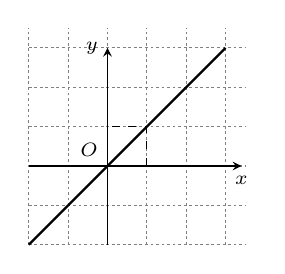
\begin{tikzpicture}[>=stealth,x=1cm,y=1cm,scale=0.5]
		\def\a{1}
		\def\b{0}
		\draw[color=gray,dash pattern=on 1pt off 1pt,xstep=1.0cm,ystep=1.0cm] (-2,-2) grid (3.5,3.5);
		\draw[->] (-2,0) -- (3.4,0) node[below] {\scriptsize $x$};
		\draw[->] (0,-2) -- (0,3) node[left] {\scriptsize $y$};
		\draw (0,0)node[above left]{\scriptsize $O$};
		\draw[thick,samples=150,smooth,domain=-2:3] plot(\x,{\a*\x+(\b)});
		\draw[dashed] (1,0) -- (1,1) -- (0,1);
		\end{tikzpicture}
	}
	{% Đồ thị hàm y=(ax+b)/(cx+d), ad-bc khác 0. Nếu hệ số lớn cần điều chỉnh hệ trục, vùng lưới, domain và lệnh \clip
		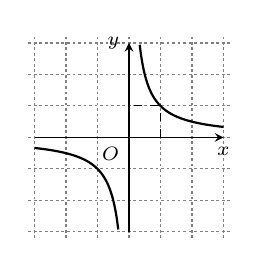
\begin{tikzpicture}[>=stealth,x=1cm,y=1cm,scale=0.4]
		\def\a{0}
		\def\b{1}
		\def\c{1}
		\def\d{0}
		\draw[color=gray,dash pattern=on 1pt off 1pt,xstep=1.0cm,ystep=1.0cm] (-3.2,-3.2) grid (3.2,3.2);
		\draw[->] (-3,0) -- (3,0) node[below] {\scriptsize $x$};
		\draw[->] (0,-3) -- (0,3) node[left] {\scriptsize $y$};
		\draw (0,0)node[below left]{\scriptsize $O$};
		\pgfmathsetmacro{\can}{-(\d)/(\c)}
		\draw[thick,samples=150,smooth,domain=-3:{\can-.34}] plot(\x,{(\a*\x+(\b))/(\c*\x+(\d))}); % Vẽ nhánh bên trái TCĐ
		\draw[thick,samples=150,smooth,domain={\can+.34}:3] plot(\x,{(\a*\x+(\b))/(\c*\x+(\d))}); % Vẽ nhánh bên phải TCĐ
		\draw[dashed] (1,0) -- (1,1) -- (0,1);
		\end{tikzpicture}
	}
	{\True 
		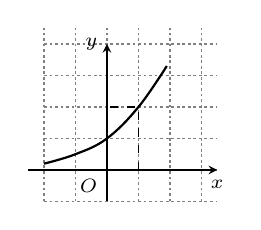
\begin{tikzpicture}[>=stealth,x=1.0cm,y=1.0cm,scale=0.4]
		\draw [color=gray,dash pattern=on 1pt off 1pt,xstep=1.0cm,ystep=1.0cm] (-2,-1) grid (3.5,4.5);
		\draw[->] (-2.5,0) -- (3.5,0) node[below] {\scriptsize $x$};
		\draw[->] (0,-1) -- (0,4) node[left] {\scriptsize $y$};
		\draw (0,0) node[below left] {\scriptsize $O$};
		\draw[thick,black] plot[smooth,tension=.65] coordinates{(-2,0.2) (-1,0.5) (0,1) (1,2) (1.9,3.3)};
		\draw[dashed] (1,0) -- (1,2) -- (0,2);
		\end{tikzpicture}
	}
	{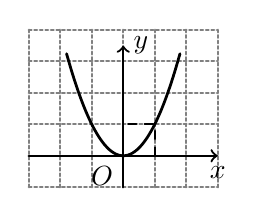
\begin{tikzpicture}[scale=0.4,line join=round, line cap=round,thick]
		\draw [color=gray,dash pattern=on 1pt off 1pt,xstep=1.0cm,ystep=1.0cm] (-3,-1) grid (3,4);
		\draw[->] (-3,0) -- (3,0)node[below]{$x$};
		\draw[->] (0,-1) -- (0,3.5)node[right]{$y$};
		\node[below left] at (0,0){$O$};
		\draw[line width=1pt,smooth,domain=-1.8:1.8]plot(\x, {(\x)^2});
		\draw[dashed] (1,0) -- (1,1) -- (0,1);
		\end{tikzpicture}}
	\loigiai{
		Đồ thị hàm số $y=x^{\alpha}$ không đi qua điểm $(0;1)$.}
\end{vd}
\begin{vd}%Ví dụ 4%[Nguyễn Diệu Linh]%[2D2Y2-3]
	Đường cong trong hình dưới đây là đồ thị hàm số nào?
	\begin{center}
		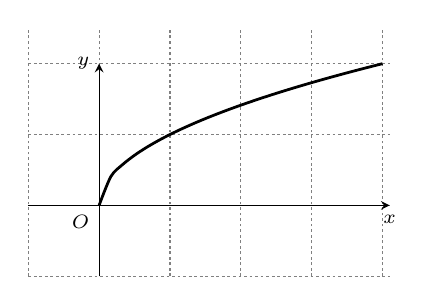
\begin{tikzpicture}[>=stealth,x=1.0cm,y=1.0cm,scale=0.9]
		\draw [color=gray,dash pattern=on 1pt off 1pt,xstep=1.0cm,ystep=1.0cm] (-1,-1) grid (4.1,2.5);
		\draw[->] (-1,0) -- (4.1,0) node[below] {\scriptsize $x$};
		\draw[->] (0,-1) -- (0,2) node[left] {\scriptsize $y$};
		\draw (0,0) node[below left] {\scriptsize $O$};
		\draw[line width=1pt,smooth,domain=0:4]plot(\x,{sqrt(\x)});
		\end{tikzpicture}
	\end{center}
	\choice
	{$y=x^{-\tfrac{1}{2}}$}
	{\True $y=x^{\tfrac{1}{2}}$}
	{$y=2^x$}
	{$y=2^{x-1}$}
	\loigiai{
		Nhận thấy đồ thị hàm số đi qua gốc tọa độ nên không thể là $y=2^x$, $y=2^{x-1}$. \\
		Nhận thấy đồ thị hàm số đi qua điểm $(4;2)$ nên không thể là $y=x^{-\tfrac{1}{2}}$.}
\end{vd}
\begin{vd}%Ví dụ 5%[Nguyễn Diệu Linh]%[2D2B2-3] 
	Cho $\alpha, \beta$ là các số thức. Đồ thị các hàm số $y=x^{\alpha}, y=x^{\beta}$ trên khoảng $(0;+\infty)$ được cho hình vẽ bên. Khẳng định nào sau đây đúng?
	\begin{center}
		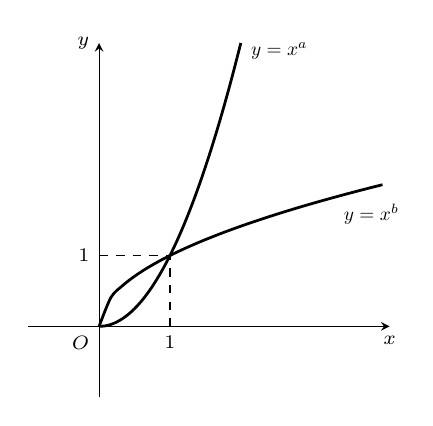
\begin{tikzpicture}[>=stealth,x=1.0cm,y=1.0cm,scale=0.9]
		\draw[->] (-1,0) -- (4.1,0) node[below] {\scriptsize $x$};
		\draw[->] (0,-1) -- (0,4) node[left] {\scriptsize $y$};
		\draw (0,0) node[below left] {\scriptsize $O$} (1,0) node[below] {\scriptsize $1$} (0,1) node[left] {\scriptsize $1$};
		\draw[line width=1pt,smooth,domain=0:2]plot(\x,{(\x)^2});
		\fill[black,every node/.style={scale=0.7}] (2.4,3.8)node[shift={(30:6pt)}]{$y=x^a$} circle (0.015pt); 
		\draw[line width=1pt,smooth,domain=0:4]plot(\x,{sqrt(\x)});
		\fill[black,every node/.style={scale=0.7}] (3.7,1.5)node[shift={(30:6pt)}]{$y=x^b$} circle (0.015pt); 
		\draw[line width=0.4pt,black,dashed] (1,0)--(1,1)--(0,1); 
		
		\end{tikzpicture}
	\end{center}
	\choice
	{$0<\beta<1<\alpha$}
	{$\beta<0<1<\alpha$}
	{$0<\alpha<1\beta$}
	{\True $\alpha<0<1<\beta$}
	\loigiai{
		Với $x_0>1$ ta có: 
		$x_0^{\alpha}>1\Rightarrow \alpha>0$;	$x_0^{\beta}>1\Rightarrow \beta>0$.\\
		Mặt khác, dựa vào hình dáng đồ thị ta suy ra $\alpha>1$ và $\beta<1$. Suy ra $\alpha<0<1<\beta$ .}
\end{vd}
\subsubsection{Câu hỏi trắc nghiệm}
\begin{ex}%Câu 1%[Nguyễn Diệu Linh]%[2D2Y2-3]
	Hình bên là đồ thị của một trong bốn hàm số dưới đây. 
	\begin{center}
		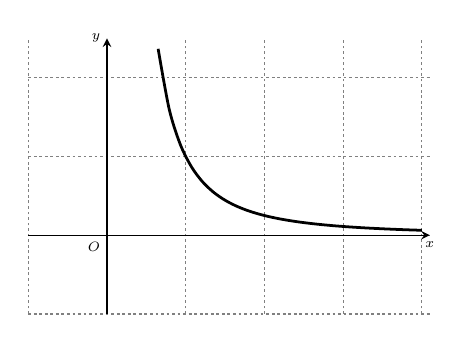
\begin{tikzpicture}[>=stealth,x=1.0cm,y=1.0cm,scale=1,every node/.style={scale=0.7}]
		\draw [color=gray,dash pattern=on 1pt off 1pt,xstep=1.0cm,ystep=1.0cm] (-1,-1) grid (4.1,2.5);
		\draw[->] (-1,0) -- (4.1,0) node[below] {\scriptsize $x$};
		\draw[->] (0,-1) -- (0,2.5) node[left] {\scriptsize $y$};
		\draw (0,0) node[below left] {\scriptsize $O$};
		\draw[line width=1pt,smooth,domain=0.65:4]plot(\x,{1/(\x)^2});
		\end{tikzpicture}
	\end{center}
	\choice
	{$y=x^{-2}$}
	{$y=2^{-x}$}
	{\True $y=x^{-\tfrac{1}{2}}$}
	{$y=\log_2x$}
	\loigiai{
		Nhận thấy đồ thị hàm số đi qua điểm $(1; 1)$ nên không thể là $y=2^{-x}$ và $y=\log_2x$ .\\
		Nhận thấy đồ thị hàm số đi qua điểm $\left(\dfrac{1}{4}; a\right), a>2$ nên không thể là $y=x^{-2}$ .}
\end{ex}
\begin{ex}%Câu 2%[Nguyễn Diệu Linh]%[2D2B2-3]
	Hình dưới đây là đồ thị của hai hàm số $y=x^a$ và $y=x^b$. Hãy chọn khẳng định đúng. 
	\begin{center}
		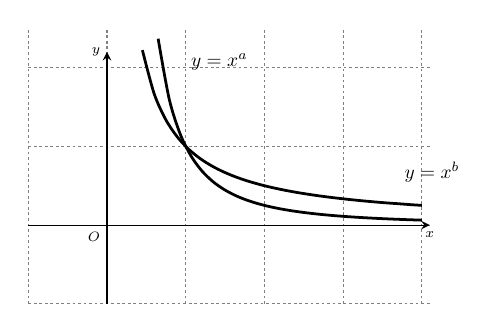
\begin{tikzpicture}[>=stealth,x=1.0cm,y=1.0cm,scale=1,every node/.style={scale=0.7}]
		\draw [color=gray,dash pattern=on 1pt off 1pt,xstep=1.0cm,ystep=1.0cm] (-1,-1) grid (4.1,2.5);
		\draw[->] (-1,0) -- (4.1,0) node[below] {\scriptsize $x$};
		\draw[->] (0,-1) -- (0,2.2) node[left] {\scriptsize $y$};
		\draw (0,0) node[below left] {\scriptsize $O$};
		\draw[line width=1pt,smooth,domain=0.45:4]plot(\x,{1/(\x)});
		\draw[line width=1pt,smooth,domain=0.65:4]plot(\x,{1/(\x)^2});
		\fill[black] (1.3,2)node[shift={(30:6pt)}]{$y=x^a$} circle (0.01pt);
		\fill[black] (4,0.6)node[shift={(30:6pt)}]{$y=x^b$} circle (0.01pt);
		
		
		\end{tikzpicture}
	\end{center}
	\choice
	{$a>b>0$}
	{$b<a<0$}
	{\True $a<b<0$}
	{$b>a>0$}
	\loigiai{
		Vì hàm số nghịch biến và
		\begin{itemize}
			\item[-] Khi $x>1$ thì $x^a<x^b\Leftrightarrow a<b$.
			\item[-]Khi $0<x<1$ thì $x^a>x^b\Leftrightarrow a<b$.
		\end{itemize}
		Do đó $a<b<0$.}
\end{ex}
\begin{ex}%Câu 3%[Nguyễn Diệu Linh]%[2D2Y2-3]
	Trong các đồ thị dưới đây, đồ thị nào là đồ thị của hàm số $y=x^{\tfrac{1}{4}}$?
	\choice
	{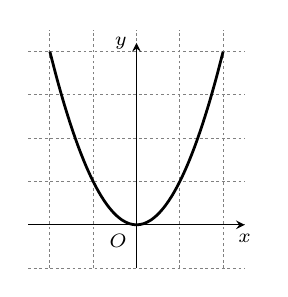
\begin{tikzpicture}[>=stealth,x=1.0cm,y=1.0cm,scale=0.55]
		\draw [color=gray,dash pattern=on 1pt off 1pt,xstep=1.0cm,ystep=1.0cm] (-2.5,-1) grid (2.5,4.5);
		\draw[->] (-2.5,0) -- (2.5,0) node[below] {\scriptsize $x$};
		\draw[->] (0,-1) -- (0,4.2) node[left] {\scriptsize $y$};
		\draw (0,0) node[below left] {\scriptsize $O$};
		\draw[line width=1pt,smooth,domain=-2:2]plot(\x,{(\x)^2});
		\end{tikzpicture}	}
	{\True 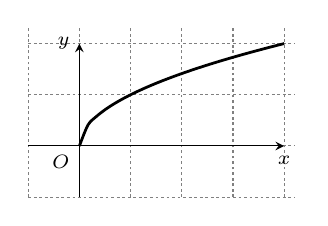
\begin{tikzpicture}[>=stealth,x=1.0cm,y=1.0cm,scale=0.65]
		\draw [color=gray,dash pattern=on 1pt off 1pt,xstep=1.0cm,ystep=1.0cm] (-1,-1) grid (4.2,2.3);
		\draw[->] (-1,0) -- (4,0) node[below] {\scriptsize $x$};
		\draw[->] (0,-1) -- (0,2) node[left] {\scriptsize $y$};
		\draw (0,0) node[below left] {\scriptsize $O$};
		\draw[line width=1pt,smooth,domain=0:4]plot(\x,{sqrt(\x)});
		\end{tikzpicture}}
	{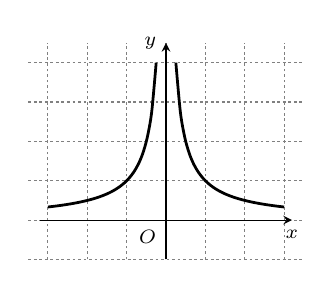
\begin{tikzpicture}[>=stealth,x=1.0cm,y=1.0cm,scale=0.5]
		\draw [color=gray,dash pattern=on 1pt off 1pt,xstep=1.0cm,ystep=1.0cm] (-3.5,-1) grid (3.5,4.5);
		\draw[->] (-3.2,0) -- (3.2,0) node[below] {\scriptsize $x$};
		\draw[->] (0,-1) -- (0,4.5) node[left] {\scriptsize $y$};
		\draw (0,0) node[below left] {\scriptsize $O$};
		\draw[line width=1pt,smooth,domain=0.25:3]plot(\x,{1/(\x)});
		\draw[line width=1pt,smooth,domain=-3:-0.25]plot(\x,{-1/(\x)});
		\end{tikzpicture}}
	{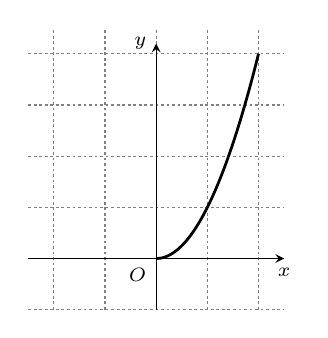
\begin{tikzpicture}[>=stealth,x=1.0cm,y=1.0cm,scale=0.65]
		\draw [color=gray,dash pattern=on 1pt off 1pt,xstep=1.0cm,ystep=1.0cm] (-2.5,-1) grid (2.5,4.5);
		\draw[->] (-2.5,0) -- (2.5,0) node[below] {\scriptsize $x$};
		\draw[->] (0,-1) -- (0,4.2) node[left] {\scriptsize $y$};
		\draw (0,0) node[below left] {\scriptsize $O$};
		\draw[line width=1pt,smooth,domain=0:2]plot(\x,{(\x)^2});
		\end{tikzpicture}}
	\loigiai{
		Do hàm số $y=x^{\tfrac{1}{4}}$ có tập xác định là $(0;+\infty)$ nên ta chỉ xét các đồ thị nằm bên phải trực tung.\\
		Mặt khác, hàm số $y=x^{\tfrac{1}{4}}$ đồng biến trên $(0;+\infty)$ nên loại D.}
\end{ex}
\begin{ex}%Câu 4%[Nguyễn Diệu Linh]%[2D2Y2-3]
	Đường cong trong hình bên là đồ thị của một hàm số trong bốn hàm số được liệt kê ở bốn phương án A, B, C, D dưới đây. Hỏi hàm số đó là hàm số nào?
	\begin{center}
		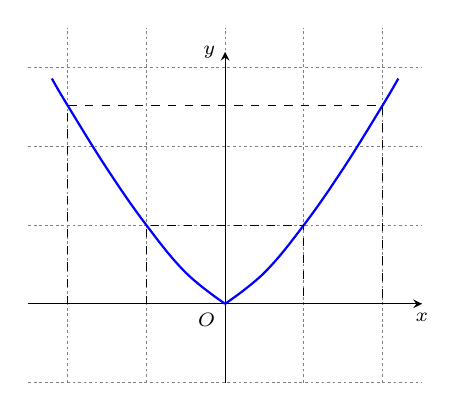
\begin{tikzpicture}[>=stealth,x=1.0cm,y=1.0cm,scale=1]
		\draw [color=gray,dash pattern=on 1pt off 1pt,xstep=1.0cm,ystep=1.0cm] (-2.5,-1) grid (2.5,3.5);
		\draw[->] (-2.5,0) -- (2.5,0) node[below] {\scriptsize $x$};
		\draw[->] (0,-1) -- (0,3.2) node[left] {\scriptsize $y$};
		\draw (0,0) node[below left] {\scriptsize $O$};
		\draw[thick,blue] plot[smooth,tension=.65] coordinates{(0,0) (0.5,0.39685) (1,1) (1.5,1.717) (2,2.51984) (2.2,2.861)};
		\draw[thick,blue] plot[smooth,tension=.65] coordinates{(-2.2,2.861) (-2,2.51984) (-1.5,1.717) (-1,1) (-0.5,0.39685) (0,0)};
		\draw[line width=0.4pt,black,dashed] (-1,0)--(-1,1)--(1,1)--(1,0) (-2,0)--(-2,2.51984)--(2,2.51984)--(2,0); % Đoạn thẳng AB
		
		
		\end{tikzpicture}	
	\end{center}
	\choice
	{\True $y=x^{\tfrac{4}{3}}$}
	{$y=x^{\tfrac{2}{3}}$}
	{$y=x^2$}
	{$y=x^4$}
	\loigiai{}
\end{ex}
\begin{ex}%Câu 5%[Nguyễn Diệu Linh]%[2D2Y2-3]
	Đường cong trong hình bên là đồ thị của một hàm số trong bốn hàm số được liệt kê ở bốn phương án A, B, C, D dưới đây. Hỏi hàm số đó là hàm số nào?
	\begin{center}
		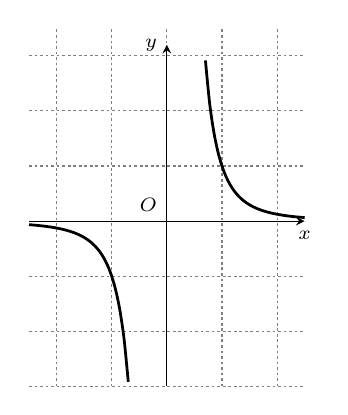
\begin{tikzpicture}[>=stealth,x=1.0cm,y=1.0cm,scale=0.7]
		\draw [color=gray,dash pattern=on 1pt off 1pt,xstep=1.0cm,ystep=1.0cm] (-2.5,-3) grid (2.5,3.5);
		\draw[->] (-2.5,0) -- (2.5,0) node[below] {\scriptsize $x$};
		\draw[->] (0,-3) -- (0,3.2) node[left] {\scriptsize $y$};
		\draw (0,0) node[above left] {\scriptsize $O$};
		\draw[line width=1pt,smooth,domain=0.7:2.5]plot(\x,{1/((\x)^3)});
		\draw[line width=1pt,smooth,domain=-2.5:-0.7]plot(\x,{1/((\x)^3)});
		
		\end{tikzpicture}	
	\end{center}
	\choice
	{\True $y=x^{-3}$}
	{$y=x^{-\tfrac{1}{3}}$}
	{$y=x^3$}
	{$y=\sqrt[3]{x}$}
	\loigiai{}
\end{ex}
\begin{ex}%Câu 6%[Nguyễn Diệu Linh]%[2D2Y2-3]
	Đường cong trong hình bên là đồ thị của hàm số
	\begin{center}
		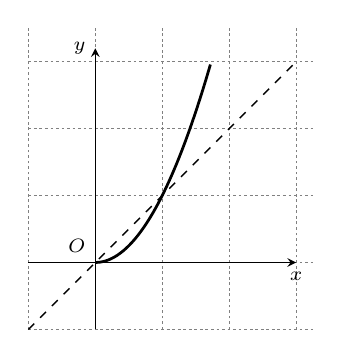
\begin{tikzpicture}[>=stealth,x=1.0cm,y=1.0cm,scale=0.85]
		\draw [color=gray,dash pattern=on 1pt off 1pt,xstep=1.0cm,ystep=1.0cm] (-1,-1) grid (3.3,3.5);
		\draw[->] (-1,0) -- (3,0) node[below] {\scriptsize $x$};
		\draw[->] (0,-1) -- (0,3.2) node[left] {\scriptsize $y$};
		\draw (0,0) node[above left] {\scriptsize $O$};
		\draw[line width=1pt,smooth,domain=0:1.72]plot(\x, {(\x)^2});
		\draw[dashed,line width=0.5pt,smooth,domain=-1:3]plot(\x, {(\x)});
		
		\end{tikzpicture}	
	\end{center}
	\choice
	{\True $y=x^{\tfrac{\pi}{2}}$}
	{$y=x^{\tfrac{1}{3}}$}
	{$y=x^{-\tfrac{5}{2}}$}
	{$y=x^{-3}$}
	\loigiai{}	
\end{ex}
\begin{ex}%Câu 7%[Nguyễn Diệu Linh]%[2D2Y2-3]
	Đường cong trong hình bên là đồ thị của hàm số
	\begin{center}
		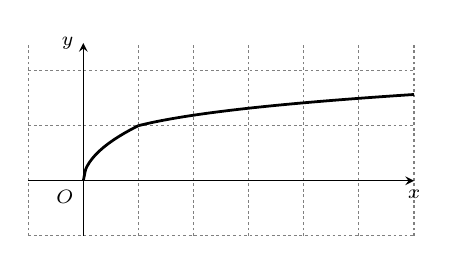
\begin{tikzpicture}[>=stealth,x=1.0cm,y=1.0cm,scale=0.7]
		\draw [color=gray,dash pattern=on 1pt off 1pt,xstep=1.0cm,ystep=1.0cm] (-1,-1) grid (6,2.5);
		\draw[->] (-1,0) -- (6,0) node[below] {\scriptsize $x$};
		\draw[->] (0,-1) -- (0,2.5) node[left] {\scriptsize $y$};
		\draw (0,0) node[below left] {\scriptsize $O$};
		\draw[line width=1pt,smooth,domain=1:6]plot(\x, {sqrt(sqrt(\x))});
		\draw[line width=1pt,smooth,domain=0:1]plot(\x, {sqrt(\x)});
		
		\end{tikzpicture}	
	\end{center}
	\choice
	{\True $y=x^{\tfrac{1}{4}}$}
	{$y=x^{-2}$}
	{$y=x^{-\tfrac{1}{3}}$}
	{$y=x^{\tfrac{3}{2}}$}	
	\loigiai{}
\end{ex}
\begin{ex}%Câu 8%[Nguyễn Diệu Linh]%[2D2B2-3]
	Hình vẽ dưới đây là đồ thị các hàm số $y=x^a,y=x^b,y=x^c$ trên miền $(0;+\infty)$. Hỏi trong các số a,b,c số nào nhận giá trị trong khoảng $(0;1)$?
	\begin{center}
		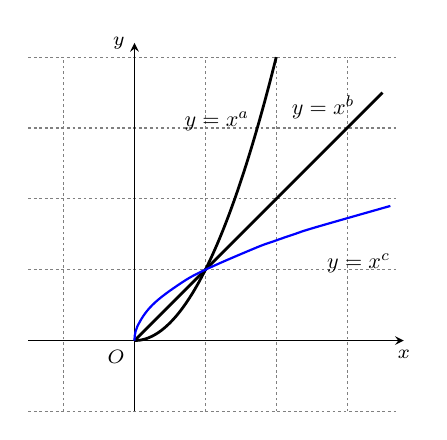
\begin{tikzpicture}[>=stealth,x=1.0cm,y=1.0cm,scale=0.9]
		\draw [color=gray,dash pattern=on 1pt off 1pt,xstep=1.0cm,ystep=1.0cm] (-1.5,-1) grid (3.7,4);
		\draw[->] (-1.5,0) -- (3.8,0) node[below] {\scriptsize $x$};
		\draw[->] (0,-1) -- (0,4.2) node[left] {\scriptsize $y$};
		\draw (0,0) node[below left] {\scriptsize $O$};
		\draw[line width=1pt,smooth,domain=0:2]plot(\x, {(\x)^2});
		\draw[line width=1pt,smooth,domain=0:3.5]plot(\x, {(\x)});
		\draw[thick,blue] plot[smooth,tension=.65] coordinates{(0,0) (0.04,0.2) (0.25,0.5) (0.64,0.8) (1,1) (1.69,1.3) (1.96,1.4) (2.25,1.5) (2.56,1.6) (3.61,1.9)};
		\fill[black,every node/.style={scale=0.8}] (1,3)node[shift={(30:6pt)}]{$y=x^a$} circle (0.01pt);
		\fill[black,every node/.style={scale=0.8}] (3,1)node[shift={(30:6pt)}]{$y=x^c$} circle (0.01pt);
		\fill[black,every node/.style={scale=0.8}] (2.5,3.2)node[shift={(30:6pt)}]{$y=x^b$} circle (0.01pt);
		
		\end{tikzpicture}
	\end{center}
	\choice
	{Số b}
	{Số a và số c}
	{\True Số c}
	{Số a}
	\loigiai{}
\end{ex}
\begin{ex}%Câu 9%[Nguyễn Diệu Linh]%[2D2B2-3]
	Hình vẽ dưới đây là đồ thị của hàm số $y=x^{\tfrac{1}{2}}$. Hỏi đồ thị của hàm số $y=|x|^{\tfrac{1}{2}}$ là hình nào?
	\begin{center}
		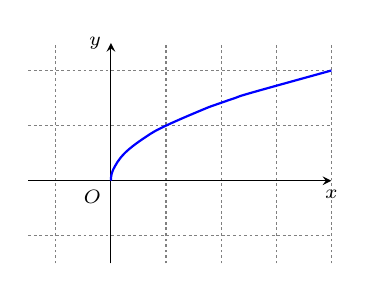
\begin{tikzpicture}[>=stealth,x=1.0cm,y=1.0cm,scale=0.7]
		\draw [color=gray,dash pattern=on 1pt off 1pt,xstep=1.0cm,ystep=1.0cm] (-1.5,-1.5) grid (4,2.5);
		\draw[->] (-1.5,0) -- (4,0) node[below] {\scriptsize $x$};
		\draw[->] (0,-1.5) -- (0,2.5) node[left] {\scriptsize $y$};
		\draw (0,0) node[below left] {\scriptsize $O$};
		\draw[thick,blue] plot[smooth,tension=.65] coordinates{(0,0) (0.04,0.2) (0.25,0.5) (0.64,0.8) (1,1) (1.69,1.3) (1.96,1.4) (2.25,1.5) (2.56,1.6) (4,2)};
		\end{tikzpicture}	
	\end{center}
	\choice
	{\True 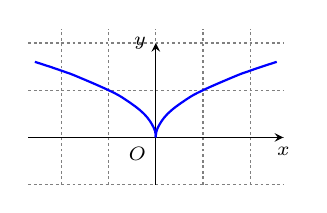
\begin{tikzpicture}[>=stealth,x=1.0cm,y=1.0cm,scale=0.6]
		\draw [color=gray,dash pattern=on 1pt off 1pt,xstep=1.0cm,ystep=1.0cm] (-2.7,-1) grid (2.7,2.3);
		\draw[->] (-2.7,0) -- (2.7,0) node[below] {\scriptsize $x$};
		\draw[->] (0,-1) -- (0,2) node[left] {\scriptsize $y$};
		\draw (0,0) node[below left] {\scriptsize $O$};
		\draw[thick,blue] plot[smooth,tension=.65] coordinates{(0,0) (0.04,0.2) (0.25,0.5) (0.64,0.8) (1,1) (1.69,1.3) (1.96,1.4) (2.25,1.5) (2.56,1.6)};
		\draw[thick,blue] plot[smooth,tension=.65] coordinates{(0,0) (-0.04,0.2) (-0.25,0.5) (-0.64,0.8) (-1,1) (-1.69,1.3) (-1.96,1.4) (-2.25,1.5) (-2.56,1.6)};
		\end{tikzpicture}}
	{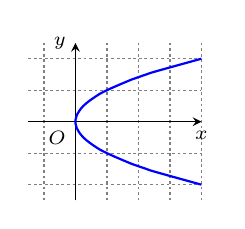
\begin{tikzpicture}[>=stealth,x=1.0cm,y=1.0cm,scale=0.4]
		\draw [color=gray,dash pattern=on 1pt off 1pt,xstep=1.0cm,ystep=1.0cm] (-1.5,-2.5) grid (4,2.5);
		\draw[->] (-1.5,0) -- (4,0) node[below] {\scriptsize $x$};
		\draw[->] (0,-2.5) -- (0,2.5) node[left] {\scriptsize $y$};
		\draw (0,0) node[below left] {\scriptsize $O$};
		\draw[thick,blue] plot[smooth,tension=.65] coordinates{(0,0) (0.04,0.2) (0.25,0.5) (0.64,0.8) (1,1) (1.69,1.3) (1.96,1.4) (2.25,1.5) (2.56,1.6) (4,2)};
		\draw[thick,blue] plot[smooth,tension=.65] coordinates{(0,0) (0.04,-0.2) (0.25,-0.5) (0.64,-0.8) (1,-1) (1.69,-1.3) (1.96,-1.4) (2.25,-1.5) (2.56,-1.6) (4,-2)};
		\end{tikzpicture}}
	{	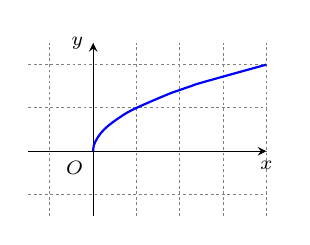
\begin{tikzpicture}[>=stealth,x=1.0cm,y=1.0cm,scale=0.55]
		\draw [color=gray,dash pattern=on 1pt off 1pt,xstep=1.0cm,ystep=1.0cm] (-1.5,-1.5) grid (4,2.5);
		\draw[->] (-1.5,0) -- (4,0) node[below] {\scriptsize $x$};
		\draw[->] (0,-1.5) -- (0,2.5) node[left] {\scriptsize $y$};
		\draw (0,0) node[below left] {\scriptsize $O$};
		\draw[thick,blue] plot[smooth,tension=.65] coordinates{(0,0) (0.04,0.2) (0.25,0.5) (0.64,0.8) (1,1) (1.69,1.3) (1.96,1.4) (2.25,1.5) (2.56,1.6) (4,2)};
		\end{tikzpicture}}
	{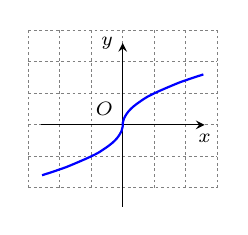
\begin{tikzpicture}[>=stealth,x=1.0cm,y=1.0cm,scale=0.4]
		\draw [color=gray,dash pattern=on 1pt off 1pt,xstep=1.0cm,ystep=1.0cm] (-3,-2) grid (3,3);
		\draw[->] (-2.6,0) -- (2.6,0) node[below] {\scriptsize $x$};
		\draw[->] (0,-2.6) -- (0,2.6) node[left] {\scriptsize $y$};
		\draw (0,0) node[above left] {\scriptsize $O$};
		\draw[thick,blue] plot[smooth,tension=.65] coordinates{(0,0) (0.04,0.2) (0.25,0.5) (0.64,0.8) (1,1) (1.69,1.3) (1.96,1.4) (2.25,1.5) (2.56,1.6)};
		\draw[thick,blue] plot[smooth,tension=.65] coordinates{(-2.56,-1.6) (-2.25,-1.5) (-1.96,-1.4) (-1.69,-1.3) (-1,-1) (-0.64,-0.8) (-0.25,-0.5) (-0.04,-0.2) (0,0)};
		\end{tikzpicture}}
	\loigiai{}
\end{ex}
\begin{ex}%Câu 10%[Nguyễn Diệu Linh]%[2D2B2-3]
	Hình vẽ dưới đây là đồ thị của hàm số $y=x^{\tfrac{1}{2}}$. Hỏi đồ thị của hàm số $y=\left|x^{\tfrac{1}{2}}\right|$ là hình nào?
	\begin{center}
		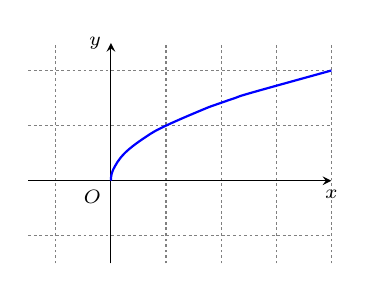
\begin{tikzpicture}[>=stealth,x=1.0cm,y=1.0cm,scale=0.7]
		\draw [color=gray,dash pattern=on 1pt off 1pt,xstep=1.0cm,ystep=1.0cm] (-1.5,-1.5) grid (4,2.5);
		\draw[->] (-1.5,0) -- (4,0) node[below] {\scriptsize $x$};
		\draw[->] (0,-1.5) -- (0,2.5) node[left] {\scriptsize $y$};
		\draw (0,0) node[below left] {\scriptsize $O$};
		\draw[thick,blue] plot[smooth,tension=.65] coordinates{(0,0) (0.04,0.2) (0.25,0.5) (0.64,0.8) (1,1) (1.69,1.3) (1.96,1.4) (2.25,1.5) (2.56,1.6) (4,2)};
		\end{tikzpicture}	
	\end{center}
	\choice
	{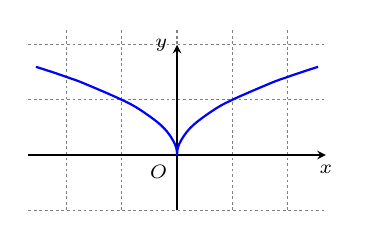
\begin{tikzpicture}[>=stealth,x=1.0cm,y=1.0cm,scale=0.7]
		\draw [color=gray,dash pattern=on 1pt off 1pt,xstep=1.0cm,ystep=1.0cm] (-2.7,-1) grid (2.7,2.3);
		\draw[->] (-2.7,0) -- (2.7,0) node[below] {\scriptsize $x$};
		\draw[->] (0,-1) -- (0,2) node[left] {\scriptsize $y$};
		\draw (0,0) node[below left] {\scriptsize $O$};
		\draw[thick,blue] plot[smooth,tension=.65] coordinates{(0,0) (0.04,0.2) (0.25,0.5) (0.64,0.8) (1,1) (1.69,1.3) (1.96,1.4) (2.25,1.5) (2.56,1.6)};
		\draw[thick,blue] plot[smooth,tension=.65] coordinates{(0,0) (-0.04,0.2) (-0.25,0.5) (-0.64,0.8) (-1,1) (-1.69,1.3) (-1.96,1.4) (-2.25,1.5) (-2.56,1.6)};
		\end{tikzpicture}}
	{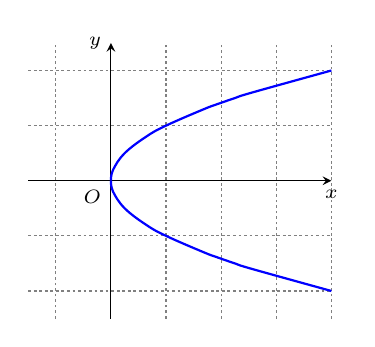
\begin{tikzpicture}[>=stealth,x=1.0cm,y=1.0cm,scale=0.7]
		\draw [color=gray,dash pattern=on 1pt off 1pt,xstep=1.0cm,ystep=1.0cm] (-1.5,-2.5) grid (4,2.5);
		\draw[->] (-1.5,0) -- (4,0) node[below] {\scriptsize $x$};
		\draw[->] (0,-2.5) -- (0,2.5) node[left] {\scriptsize $y$};
		\draw (0,0) node[below left] {\scriptsize $O$};
		\draw[thick,blue] plot[smooth,tension=.65] coordinates{(0,0) (0.04,0.2) (0.25,0.5) (0.64,0.8) (1,1) (1.69,1.3) (1.96,1.4) (2.25,1.5) (2.56,1.6) (4,2)};
		\draw[thick,blue] plot[smooth,tension=.65] coordinates{(0,0) (0.04,-0.2) (0.25,-0.5) (0.64,-0.8) (1,-1) (1.69,-1.3) (1.96,-1.4) (2.25,-1.5) (2.56,-1.6) (4,-2)};
		\end{tikzpicture}}
	{\True 	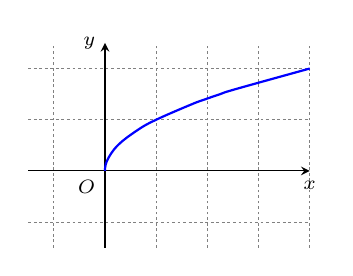
\begin{tikzpicture}[>=stealth,x=1.0cm,y=1.0cm,scale=0.65]
		\draw [color=gray,dash pattern=on 1pt off 1pt,xstep=1.0cm,ystep=1.0cm] (-1.5,-1.5) grid (4,2.5);
		\draw[->] (-1.5,0) -- (4,0) node[below] {\scriptsize $x$};
		\draw[->] (0,-1.5) -- (0,2.5) node[left] {\scriptsize $y$};
		\draw (0,0) node[below left] {\scriptsize $O$};
		\draw[thick,blue] plot[smooth,tension=.65] coordinates{(0,0) (0.04,0.2) (0.25,0.5) (0.64,0.8) (1,1) (1.69,1.3) (1.96,1.4) (2.25,1.5) (2.56,1.6) (4,2)};
		\end{tikzpicture}}
	{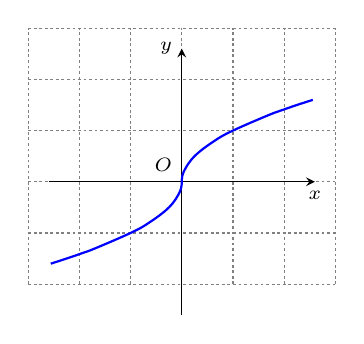
\begin{tikzpicture}[>=stealth,x=1.0cm,y=1.0cm,scale=0.65]
		\draw [color=gray,dash pattern=on 1pt off 1pt,xstep=1.0cm,ystep=1.0cm] (-3,-2) grid (3,3);
		\draw[->] (-2.6,0) -- (2.6,0) node[below] {\scriptsize $x$};
		\draw[->] (0,-2.6) -- (0,2.6) node[left] {\scriptsize $y$};
		\draw (0,0) node[above left] {\scriptsize $O$};
		\draw[thick,blue] plot[smooth,tension=.65] coordinates{(0,0) (0.04,0.2) (0.25,0.5) (0.64,0.8) (1,1) (1.69,1.3) (1.96,1.4) (2.25,1.5) (2.56,1.6)};
		\draw[thick,blue] plot[smooth,tension=.65] coordinates{(-2.56,-1.6) (-2.25,-1.5) (-1.96,-1.4) (-1.69,-1.3) (-1,-1) (-0.64,-0.8) (-0.25,-0.5) (-0.04,-0.2) (0,0)};
		\end{tikzpicture}}
	\loigiai{}
\end{ex}
\begin{ex}%Câu 11%[Nguyễn Diệu Linh]%[2D2B2-3]
	Hình vẽ dưới đây là đồ thị của hàm số $y=x^{\tfrac{1}{2}}$. Hỏi đồ thị của hàm số $y=\left|x^{\tfrac{1}{2}}-1\right|$ là hình nào?
	\begin{center}
		
		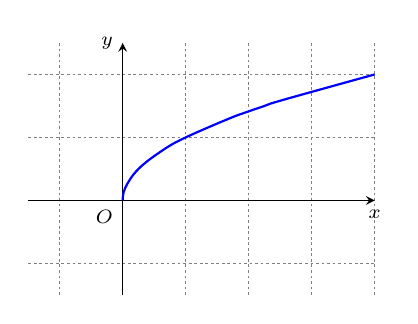
\begin{tikzpicture}[>=stealth,x=1.0cm,y=1.0cm,scale=0.8]
		\draw [color=gray,dash pattern=on 1pt off 1pt,xstep=1.0cm,ystep=1.0cm] (-1.5,-1.5) grid (4,2.5);
		\draw[->] (-1.5,0) -- (4,0) node[below] {\scriptsize $x$};
		\draw[->] (0,-1.5) -- (0,2.5) node[left] {\scriptsize $y$};
		\draw (0,0) node[below left] {\scriptsize $O$};
		\draw[thick,blue] plot[smooth,tension=.65] coordinates{(0,0) (0.04,0.2) (0.25,0.5) (0.64,0.8) (1,1) (1.69,1.3) (1.96,1.4) (2.25,1.5) (2.56,1.6) (4,2)};
		\end{tikzpicture}
		
	\end{center}
	\choice
	{	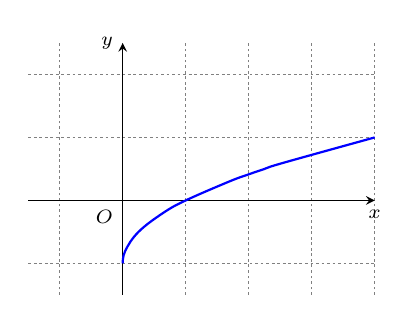
\begin{tikzpicture}[>=stealth,x=1.0cm,y=1.0cm,scale=0.8]
		\draw [color=gray,dash pattern=on 1pt off 1pt,xstep=1.0cm,ystep=1.0cm] (-1.5,-1.5) grid (4,2.5);
		\draw[->] (-1.5,0) -- (4,0) node[below] {\scriptsize $x$};
		\draw[->] (0,-1.5) -- (0,2.5) node[left] {\scriptsize $y$};
		\draw (0,0) node[below left] {\scriptsize $O$};
		\draw[thick,blue] plot[smooth,tension=.65] coordinates{(0,-1) (0.04,-0.8) (0.25,-0.5) (0.64,-0.2) (1,0) (1.69,0.3) (1.96,0.4) (2.25,0.5) (2.56,0.6) (4,1)};
		\end{tikzpicture}}
	{\True 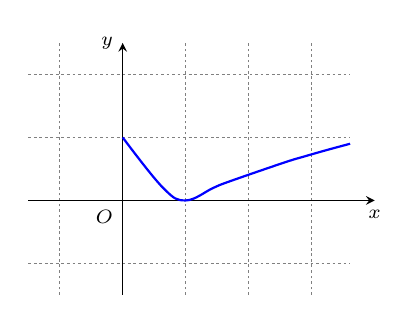
\begin{tikzpicture}[>=stealth,x=1.0cm,y=1.0cm,scale=0.8]
		\draw [color=gray,dash pattern=on 1pt off 1pt,xstep=1.0cm,ystep=1.0cm] (-1.5,-1.5) grid (3.61,2.5);
		\draw[->] (-1.5,0) -- (4,0) node[below] {\scriptsize $x$};
		\draw[->] (0,-1.5) -- (0,2.5) node[left] {\scriptsize $y$};
		\draw (0,0) node[below left] {\scriptsize $O$};
		\draw[thick,blue] plot[smooth,tension=.65] coordinates{(0,1) (0.64,0.2) (1,0) (1.44,0.2) (1.69,0.3) (2.56,0.6) (2.89,0.7) (3.24,0.8) (3.61,0.9)};
		\end{tikzpicture}}
	{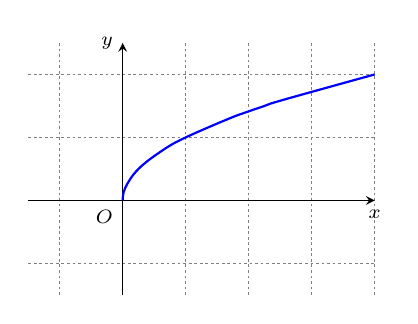
\begin{tikzpicture}[>=stealth,x=1.0cm,y=1.0cm,scale=0.8]
		\draw [color=gray,dash pattern=on 1pt off 1pt,xstep=1.0cm,ystep=1.0cm] (-1.5,-1.5) grid (4,2.5);
		\draw[->] (-1.5,0) -- (4,0) node[below] {\scriptsize $x$};
		\draw[->] (0,-1.5) -- (0,2.5) node[left] {\scriptsize $y$};
		\draw (0,0) node[below left] {\scriptsize $O$};
		\draw[thick,blue] plot[smooth,tension=.65] coordinates{(0,0) (0.04,0.2) (0.25,0.5) (0.64,0.8) (1,1) (1.69,1.3) (1.96,1.4) (2.25,1.5) (2.56,1.6) (4,2)};
		\end{tikzpicture}}
	{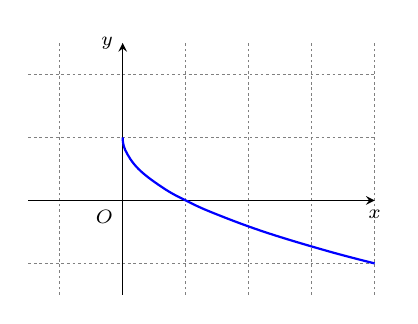
\begin{tikzpicture}[>=stealth,x=1.0cm,y=1.0cm,scale=0.8]
		\draw [color=gray,dash pattern=on 1pt off 1pt,xstep=1.0cm,ystep=1.0cm] (-1.5,-1.5) grid (4,2.5);
		\draw[->] (-1.5,0) -- (4,0) node[below] {\scriptsize $x$};
		\draw[->] (0,-1.5) -- (0,2.5) node[left] {\scriptsize $y$};
		\draw (0,0) node[below left] {\scriptsize $O$};
		\draw[thick,blue] plot[smooth,tension=.65] coordinates{(4,-1) (3.24,-0.8) (2.25,-0.5) (1.44,-0.2) (1,0) (0.64,0.2) (0.25,0.5) (0.04,0.8) (0,1)};
		\end{tikzpicture}}
	\loigiai{}
	
\end{ex}
\Closesolutionfile{ans}
%\begin{indapan}
%	{10}{ans/ansCD2D2-2}
%\end{indapan}